%% Author_tex.tex
%% V1.0
%% 2012/13/12
%% developed by Techset
%%
%% This file describes the coding for rsproca.cls

\documentclass[]{rsos}%%%%where rsos is the template name

\usepackage{wasysym}
\usepackage{caption}
\usepackage{subcaption}
\usepackage{lineno}
\linenumbers

%%%% *** Do not adjust lengths that control margins, column widths, etc. ***

%%%%%%%%%%% Defining Enunciations  %%%%%%%%%%%
\newtheorem{theorem}{\bf Theorem}[section]
\newtheorem{condition}{\bf Condition}[section]
\newtheorem{corollary}{\bf Corollary}[section]
%%%%%%%%%%%%%%%%%%%%%%%%%%%%%%%%%%%%%%%%%%%%%%%


\begin{document}

%%%% Article title to be placed here
\title{Decoding the dynamics of dental distributions: insights from shark demography and dispersal}

% Can we sneak a Jaws reference here? like "It's a squal us" or "Smile" or something about a need for a "bigger boat" or something about "going fishing" or a "toothy problem". OR: Show me your teeth: determining demography.... what about: Decoding the dynamics of dental distributions with demographic 

\author{%%%% Author details
Sora L. Kim$^{1,2,*}$, Justin D. Yeakel$^{1,*}$, Meghan Balk$^{3}$, Jaelyn J. Eberle$^{4}$, Sarah Zeichner$^{2,5}$, Dina Fieman$^{6}$, J\"urgen Kriwet$^{7}$}
% and X. Third author$^{3}$}%

%%%%%%%%% Insert author address here
\address{\footnotesize{$^{1}$School of Natural Science, University of California Merced,$^{2}$Department of Geophysical Sciences, University of Chicago, $^{3}$National Ecological Observatory Network, $^{4}$Department of Geological Sciences and Museum of Natural History, University of Colorado,
$^{5}$Division of Geological and Planetary Sciences, California Institute of Technology, $^{6}$School of Geography, Environment, and Earth Sciences, Victoria University of Wellington, $^{7}$Department of Paleontology, University of Vienna
$^{*}$Contributed equally}}


%%%% Subject entries to be placed here %%%%
\subject{paleontology, ecology, body size, migration, nursery}

%%%% Keyword entries to be placed here %%%%
\keywords{sand tiger, metapopulation, Eocene, Gulf of Mexico, Arctic, Antarctic, Delaware Bay, latitudinal gradient, body size}

%%%% Insert corresponding author and its email address}
\corres{Sora Kim\\
\email{skim380@ucmerced.edu}}

%%%% Abstract text to be placed here %%%%%%%%%%%%
\begin{abstract} %200 words max
Shark teeth are the most abundant vertebrate fossil, and because tooth size generally correlates with body size, their accumulations document the size structure of populations. Understanding how ecological and environmental processes influence size structure, and how this extends to influence these dental distributions, may offer a window into the ecological and environmental dynamics of past and present shark populations. Here we examine the dental distributions of sand tigers, including extant \emph{Carcharias taurus} and extinct \emph{Striatolamia macrota}, to reconstruct the  size structure for a contemporary locality and four Eocene localities. We compare empirical distributions against expectations from a population simulation to gain insight into potential governing ecological processes. Specifically, we investigate the influence of dispersal flexibility to and from protected nurseries. We show that changing the flexibility of initial dispersal of juveniles from the nursery and annual migration of adults to the nursery explains a large amount of dental distribution variability. Our framework predicts dispersal strategies of an extant sand tiger population, and supports nurseries as important components of sand tiger life history in both extant and Eocene populations. These results suggest nursery protection may be vital for shark conservation with increasing anthropogenic impacts and climate change.
\end{abstract}
%%%%%%%%%%%%%%%%%%%%%%%%%%%


\maketitle

\section{Introduction}
% Extant sharks occupy a wide range of habitats varying from fresh, brackish, and saline waters as well as all oceanic basins except the Southern Ocean of Antarctica.

Sharks have been a cornerstone of oceanic communities for hundreds of millions of years, a rare constant in a sea of change.
The enormous spatial and temporal dominance of shark species suggests considerable ecological plasticity, which has likely contributed to their evolutionary success and may be key to understanding the ongoing and future effects of climate change on this diverse group.
%Fossil shark teeth are the most abundant vertebrate fossil and often the only element for paleoecological studies since their skeletal tissue rarely withstand fossilization.
Documenting the success of sharks as marine predators has followed a trail of fossilized teeth, accumulating in ocean sediments and indirectly recording their ecological variability as well as the oceanic conditions in which they lived.
%Inferences to ecological and environmental processes are difficult to deduce from fossils because the large spatial and temporal distribution of the recorded data. 
While shark teeth are the most abundant vertebrate fossil, with a record spanning over 400 million years, the dynamics giving rise to these dental distributions -- in particular the interacting effects of shark ecology and the environment -- are not well understood.
% These ecological and evolutionary traits hint that sharks are resilient to climate change; however, an integrated risk assessment for sharks and rays in the Great Barrier Reef suggests those in coastal areas with freshwater inputs are most vulnerable due to changes in temperature, salinity, and ocean circulation \cite{Chin2010}.

%Tooth distributions to body size
The geologic record is prolific with fossil shark teeth as well as dermal denticles, both of which document past shark populations and community by way of accumulation. 
Collections of this material are well-suited to provide insight into the biological organization of shark communities across large spatial and temporal scales.
% These specimens provide insight into shark ecology and environmental conditions with the potential for quantitative analysis examining biological organization on larger spatial and temporal scales.
For example, collections of dermal denticles have provided insight into how shark community composition responded to the Cretaceous- Paleogene mass extinction \cite{sibert2018two}, and revealed a severe loss of shark diversity or range shift during the early Miocene \cite{sibert2021early, naylor2021comment, feichtinger2021comment}.
It is possible that accumulations of shark teeth within narrow temporal windows can  provide insights to the functioning of shark populations and communities because tooth size scales allometrically with body size \cite{Shimada2002, Shimada2004, Shimada2007}.
% For example, oxygen isotope analysis of shark enameloid indicates tolerance across a large temperature and salinity range \cite{Kim2014d, Kim2020}, 
While fossil shark teeth assemblages have been used to elucidate water temperature and salinity \cite{Kim2014d, zacke2009surface} as well as species' age distributions \cite{Kim2020}, ontogenetic stages \cite{straube2020intraspecific}, and the presence of nurseries \cite{Pimiento2010, herraiz2020use, Villafana2020}, the ecological mechanisms driving population size structure remain enigmatic even in extant populations.


% , when distributions are taken across species, and populations, when distributions are taken within species.
%I'm going to see how moving the 'here we' statement a bit forward works, as I don't think we've built up to the mystery that comes before we state the mystery we are trying to solve!
% Here, we seek to delve further into ecology by exploring how body size distributions project ecological interactions and traits as well as environmental condition in sharks.
% INSERT: something related to examples of overcoming or altering distribution to salinity / oxygen change.

% Body size to life history back to tooth distributions to the past
%Sharks are gape-limited predators, meaning that body size has an enormous influence on the structure and functioning of the higher trophic levels of marine communities \cite{brose2006consumer}. 
Body size has an enormous influence on the structure and functioning of marine communities \cite{brose2006consumer}. 
Sharks are gape-limited predators, and gape size scales with body size.
Following birth, individuals must acquire enough energy to both build and maintain somatic tissue, achieving reproductive maturity and eventually reaching an asymptotic body size \cite{West:2001bv}.
Because the majority of shark species are ectothermic, the rate at which individuals grow is constrained not only by resource availability \cite{bhat2020scaling}, but also by water temperature \cite{schindler2002sharks}. 
As temperature varies seasonally and spatially, shark species that migrate between regions are subject to changing growth rates as they transition from juvenile to adult size classes \cite{heithaus2007nursery,doan2020adult}, and some species may integrate behaviors that take advantage of differentials in resources and temperature to escape smaller body sizes more quickly.
For example, many contemporary shark species give birth in warmer estuarine environments where resources are plentiful and large predators are rare, whereupon individuals migrate to colder pelagic environments as they grow \cite{heupel2007shark}.
Such life history processes, especially those contributing to dispersal over time and space, will affect their imprint on the dental distributions left behind, and may be one of the few windows into the ecologies of ancient shark species, as well as their relationships to past climates.
% Because tooth distributions are often preserved across paleontological timescales, it is possible that the ecological mechanisms from which they arise can be explored, providing insight into the processes that led to their accumulation.


% Body size is a biological indicator often used to determine ontogeny and energy balance in mammals and fish. 
% % in sharks, body size is related to tooth crown height where, when comparing the same tooth position, smaller teeth are associated with smaller individuals \cite{Shimada2002, Shimada2004, Shimada2007, Shimada2020, Villafana2020}.
% Body size distributions of species within a geographic area are controlled by a combination of biotic interactions [e.g., in plants (Muller-Landau et al. 2006; West et al. 2006)] and resource acquisition (Kerr and Dickie 2001; Ernest et al. 2003).
% Less known are controls on body size distributions of a species across its geographic range.
% In fish, in addition to resources and biotic controls, temperature plays an important role in determining growth speed and asymptotic size. 
% % One way to probe the interaction between biology and environment when interpreting  body size distributions is to look at theoretical models that factor life history and temperature.
% % These dynamic model outputs can be compared to empirical data to infer processes and mechanisms that shape body size distributions.

%THE PAST: THE EOCENE
%NOTE: I think we should save the 'We did x,y' for the paragraph below starting 'Here we', as this still reads a background and sets us up for what we do
% We chose to examine the impacts of environment on shark population structure in the Eocene given their prolific fossil record and abundance in archived collections.  
The Eocene (56-33.9 Ma) is known for its abundant shark fossil record, with archived collections spanning locations that range from the equator to both poles.
%since To understand the effects of the current climate crisis, much insight can be gained from reconstructing shark paleobiology 
This time period may represent a deep-time analogue for the current climate crisis \cite{burke2018pliocene}, perhaps facilitating a better understanding of how contemporary shark species might respond to similar environmental pressures.
Sand tigers occupied a nearly continuous latitudinal gradient ranging from the Arctic to Southern Ocean in the Eocene, demonstrating their remarkable plasticity. 
The sole evidence of their vast geographical distribution and evolutionary success is contained within local collections of fossilized teeth.
For example, high-latitude sites such as Banks Island were deltaic, brackish zones in the Canadian Arctic with reduced salinity \cite{Waddell2008, Kim2014d} and low shark diversity \cite{greenwood2010wet, padilla2014sand}(figure \ref{fig:map}, dark green), whereas sites such as Seymour Island off the Antarctic Peninsula were fully marine  habitats \cite{Ivany2008} with high shark diversity \cite{Long1992,Kriwet2016, Kriwet2005,Reguero2012,Engelbrecht2019} (figure \ref{fig:map}, dark blue).
Despite these environmental differences, sand tigers  (${}^\dag$\emph{Striatolamia macrota}, Agassiz, 1843 and ${}^\dag$\emph{Carcharias macrota}; extinct species denoted with ${}^\dag$) occupied both locales during the Eocene \cite{Kriwet2005,Reguero2012,Padilla2014,Kriwet2016,Engelbrecht2019,purdy1998chondrichthyan}, in addition to lower latitude environments, notably in the Gulf of Mexico \cite{Westgate}(figure \ref{fig:map}, lighter shades).
% which share many characteristics and are synonymized by some \cite{purdy1998chondrichthyan}.
% We chose two mid-latitude localities because their community assemblage resembled the those in high latitudes.
Low latitude Eocene sites exhibit an environmental gradient similar to that of the high latitude sites, but in warmer waters with less seasonal variability.
For example, the low latitude Red Hot Truck Stop locality of the Tuscahoma and Bashi formations (Fm) in Mississippi was a reduced salinity habitat \cite{ingram1991tuscahoma,Beard2009} (figure \ref{fig:map}, light green), similar to that of Banks Island in the Arctic, whereas the Whiskey Bridge locality of the Crockett Fm. in Texas reflected a more diverse assemblage characteristic of pelagic communities \cite{Breard1999,Westgate,harding2014mineralogy}(figure \ref{fig:map}, light blue), bearing greater similarity with Seymour Island in the Southern Ocean (figure \ref{fig:map}). 
% In contrast, the Stone City Fm. at Whiskey Creek Bridge is dominated by marine fauna and sediments indicate a sheltered, 20-60m depth micro-tidal sea subject to repetitive hurricane-intensity storm disturbance . 
Compellingly, these dental distributions reveal unique and idiosyncratic attributes, which may encode important ecological relationships governing Eocene sand tiger populations.
% and fossil teeth provide biologically relevant data that allow comparisons among populations and insight to ecological plasticity.

%Body size is an often measured biological trait because it reflects an organism's energy balance, for which there are different demands related to ontogeny and environment. 
% Body size is thought to increase with latitude for endothermic taxa (i.e., birds and mammals); however, there is mixed evidence for ectotherms and even differing patterns at the generic and species level. 
% A review of freshwater fishes suggests an inverse Bergmann’s Rule \cite{Belk2002}, but this hypothesis is difficult to test for sharks today given the low diversity in the Arctic Ocean (i.e., only Greenland sharks) and lack of species in today’s Southern Ocean. 
% [MAB NOTE: I think we stay away from Bergmann's Rule only because this paper doesn't really test it and because there isn't a temperature gradient.] SLK: deleted that bit

Here we examine sand tiger dental distributions from these four Eocene localities that span high- and low-latitudes, as well as a contemporary sand tiger population near Delaware Bay (figure \ref{fig:map}).
We observe that shark dental distributions vary not only in terms of means and variance, but that some reveal pronounced bimodality while others do not.
% Such bimodality is a common feature of shark tooth size distributions, and while in for some species may be related to sexual dimorphism, for others - including sand tiger sharks - 
Given that tooth size and body size are strongly correlated \cite{Shimada2002, Shimada2004, Shimada2007}, such variation in the shapes of local dental distributions may reflect an intersection of environmental and ecological drivers contributing to the presence of different shark size classes in each locality.
For example, many shark species migrate to coastal nurseries to reproduce \cite{Jorgensen2010,Macdonald2021} and the increased concentration of juveniles at these sites may skew dental distributions to smaller sizes compared to sites in pelagic environments with a higher proportion of adults.

We next assess how temperature, seasonality, and dispersal to and from a nursery, or juvenile, site can affect the shapes of dental distributions.
To investigate these effects, we constructed a mechanistic model of a two-site shark metapopulation, where one site serves as a coastal nursery (the juvenile site) and the other serves as a pelagic adult habitat (the adult site) (figure \ref{fig:diagram}). 
Our population-level framework incorporates temperature-dependent growth, size-dependent first dispersal of juveniles from the nursery to the adult site, and the seasonal dispersal of adults from the pelagic adult site to the coastal nursery.
Comparing observed dental distributions to those generated by our model enables a disentangling of likely ecological and environmental mechanisms contributing to observed differences in dental distribution geometries.

Our results point to three key findings.
First, we show that changing the flexibility of initial juvenile dispersal to the adult site and annual adult dispersal to the juvenile site have a large effect on dental distribution shape, impacting the mean, variance, and presence or absence of bimodality, all of which feature into shaping empirical distributions.
Second, we leverage our framework to correctly predict whether a contemporary sand tiger size structure represents either a juvenile or adult locality, as well as aspects of known life history traits characterizing the dispersal habits of sand tigers occupying the Delaware Bay.
Third, we show that our framework, when applied to both contemporary and Eocene sand tiger populations, emphasizes the importance of seasonal adult dispersal as well as the role of juvenile sites serving as nursery localities from the Eocene to the present in both high- and low-latitude localities.
That our results support the presence of shark nurseries across a range of oceanic conditions spanning ~50 million years lends particular credence to the notion that protecting nursery sites may be vital for shark conservation in the face of future climate change.

% That our approach both supports our understanding of a contemporary sand tiger population 

% [1 - dental distribution in contemporary in eocene communities are diverse]
% [2 - basic life history characteristics controlling dispersal to, from juvenile and adult sites result in a large diversity of dental distribution geometries]
% [3 - we can gain mechanistic insight into the drivers of contemporary dental distributions by back-calculating life history characteristics from distribution shape]
% [4 - use this to gain insight into the ecologies of eocene populations spanning the poles]



% each empirical site has a unique/idiosyncratic distribution that can't be attributed to temp/location
% the mean of nursery and adult dental distributions can vary enormously, depending on how well sites are 'mixed'
% The juvenile and adult migration windows have the largest effect on this 'mixing', largely determining changes in mean and whether or not the distributions exhibit bimodality
% Bimodality (in both site types) is the consequence of increased variability of when a juvenile transitions adult site (high mixing of juveniles), and more strict seasonality for when adults reproduce at the nursery (low mixing of adults).
% Finally we explore best fits and show that, given model assumptions, some sites can be more readily distinguished as juv/adult, whereas for others it is more uncertain
% Tusc/Banks are more similar environs and both are good fits for juvenile sites despite having distributions that look different... both have small juv migration windows and low to intermediate adult migration windows
% StoneCity/Antarctica are more similar environs but have different migrational interpretations. StoneCity more likely adult site; Antarctica could be either (a juv site with high adult migration window and low juv adult migration window... or an adult site with high juv and high adult migraiton windows). 


% I THINK SOME OF THE ORIGINAL INTRO MATERIAL MIGHT BE BETTER IN DISCUSSION...
%I'VE MOVED IT TO DISCUSSION



\section{Methods}

%\subsection{Geologic Setting}
%\underline{Banks Island, NWT Canada}
%The fossil shark teeth from the Arctic were discovered as float on the unconsolidated Cyclic Member sands of the Eureka Sound Formation close to the Muskox and Eames rivers within Aulavik National Park on northern Banks Island, Northwest Territories (NWT), Canada (~74o N). 
%Researchers should request the exact coordinates from the Canadian Museum of Nature, Ottawa, Canada. 
%The fossil shark teeth localities near the Muskox and Eames rivers are Eocene in age. This is based on pollen samples, mammalian biostratigraphy, and a zircon produced date of 〖52.6〗\pm 1.9 Ma \cite{Miall1979, Sweet2012, Reinhardt2010, Hopkins1974, Hopkins1975}. 

%\underline{Seymour Island, Antarctica}
%The Antarctic shark teeth are from the La Meseta Formation on Seymour Island, 100 km east of the Antarctic Peninsula at 64°17’S, 56°45’W \cite{Sadler1988, Ivany2008, Kriwet2005, Kriwet2016, Engelbrecht2017, Engelbrecht2017b, Engelbrecht2017c, Engelbrecht2017d, Engelbrecht2019}. 
%Previous studies estimate that La Meseta Fm. spans Early – early Middle Eocene to Late Eocene, with TELMs 2-5, which contain \emph{S. macrota} teeth, spanning ~early Middle Eocene to Late Middle Eocene \cite{Long1992, Stilwell1992, Reguero2012, Kriwet2016}    
%Previous studies have determined that the La Meseta Fm. depositional environment was estuarine \cite{Marenssi1994, Ivany2008, Amenabar2020}.

%\underline{Whiskey Bridge, Burleston County, TX USA}
%The shark teeth from Texas were found in the Stone City Formation (~41.8Ma), which is located on the south bank of the Brazos River in Burleston County, TX, 18.5km west of Bryan, Brazos County, TX \cite{Breard1999, Westgate} (and personal correspondence with C.J. Flis, Oct. 2016). 
%Stone City Fm.’s late Middle Eocene age was determined by biostratigraphy and radiometric dating of nearby fossil ash (Heintz et al., 2015; personal correspondence with C.J. Flis, Oct. 2016).
%Previous studies of Stone City Fm. sediment deposition suggest a sheltered, 20-60m depth micro-tidal sea subject to repetitive hurricane-intensity storm disturbance \cite{Breard1999, harding2014mineralogy} (and personal correspondence with C.J. Flis, Oct. 2016).  

%\underline{Red Hot Truck Stop, Meridian, Mississippi}
%The shark teeth found in eastern Mississippi were discovered in the unconsolidated sands of the T4 Channel Sand at the top of Tuscahoma Fm. at the Red Hot Truck Stop locality (Carnegie Museum or CM 517), near Interstate 20, in the NW corner, of the NW ¼, of the NE ¼, of Section 20, T6N, R16E, Lauderdale County, Mississippi \cite{ingram1991tuscahoma}. 
%At the base of the T4 Sand is a lag deposit that preserved the vertebrate teeth and fossil fragments (Ingram, 1991). The upper Tuscahoma T4 sand was dated to be 55-+ 1.4 Ma \cite{mancini1995geochronology} using potassium-argon (K-Ar) radiometric age determination.
%The lithology of the Tuscahoma Formation and T4 Sand is consistent with that of a large-scale, fluvial-dominated deltaic system \cite{Beard2009}. 

\subsection{Tooth Identification and Measurement}
Shark species in the fossil record are largely identified by their tooth morphology \cite{Cappetta2012} due to the poor preservation of cartilaginous skeletons. 
${}^\dag$\emph{Striatolamia macrota} teeth are identified by emphasized striations on the lingual side relative to the smooth labial side \cite{Cappetta2012}. 
Anterior teeth (A1-2 and a1-2) are recognized by their long and narrow shape, compared to the lateral and posterior teeth that have a short, blade-like appearance \cite{Cunningham2000}. 
The anterior teeth have an acute angle between the two roots and have two small lateral cusplets \cite{Padilla2014, Cappetta2012}. 
This tooth position was chosen as a proxy for body size because its large size and distinct morphology compared to other tooth positions within the jaw. 
Limiting the positions measured from fossil teeth prevents potential for over representation of a single individual within the assemblage. 
%Because the shark body length and tooth crown height relationship established by Shimada \cite{Shimada2004} for \emph{C. taurus} may not be representative and accurate for the Eocene species ${}^\dag$\emph{S. macrota}, we reconstruct body length using anterior crown height. 
We measured anterior tooth height from the enameloid base to the blade tip with digital calipers to an accuracy of 0.1 mm. 
The labial and lingual sides of the tooth, and the maximum width was also measured and recorded. 
The labial side of the tooth is adjacent to the cheek of the shark, and the lingual is that side adjacent to the tongue \cite{Cappetta2012}.  
Every seventh tooth was re-measured for 0.3 mm accuracy. 

%To ground truth the population model, we  used total length measurements from an extant \emph{Carcharias taurus} population tagged near Delaware Bay, USA \cite{Teter2015}. 
The modern analogue for the Eocene ${}^\dag$\emph{S. macrota} is the extant sand tiger \emph{C. taurus} based on the similarities in tooth shape throughout the entire dentition \cite{Cunningham2000}. 
We transformed total length measurements from the 2012 tagging season in Delaware Bay \cite{haulsee2016implantation, haulsee2018spatial, Teter2015, kilfoil2017targeted} to anterior tooth crown height based on the allometric relationships from Shimada et al. \cite{Shimada2002} and previously applied to fossil \emph{S. macrota} in Kim et al. \cite{Kim2020}. %12.50 * ATCH - 26.24 = TL where ATCH is the anterior tooth crown height of A1-2 and a1-2 using data in Shimada \cite{Shimada2002} and previously applied to fossil \emph{S. macrota} in Kim et al. \cite{Kim2020}. 
% Given the extensive knowledge of this contemporary population's movement patterns in the western Atlantic from Massachusetts to Florida \cite{haulsee2018spatial, Teter2015, Kneebone2012, kneebone2014movement}, this body size distribution provided a qualitative metric for the model's accuracy.

For each assemblage, we tested the sample size needed to estimate the mean and standard deviation of the tooth distribution. 
We then calculated the means and standard deviations of each tooth distribution and performed a power test to calculate the sample size required to estimate the mean and standard deviation within a 95\% confidence level and 10\% margin of error. 

%Sharks replace teeth throughout their lifetime with a conveyor belt-like system. 
%In many modern sharks, including sand tigers, teeth within an individual position scale with body size \cite{Shimada2002, Shimada2004, Shimada2007, Shimada2020}. 
%We used anterior tooth height as a proxy for body size and interpret population size distribution for \emph{Striatolamia macrota} in each locality. 
${}^\dag$\emph{Striatolamia macrota} teeth from Banks Island are curated at the Canadian Museum of Nature (Ottawa, ON Canada); Seymour Island are curated at the University of California Museum of Paleontology (UCMP; Berkeley, CA USA), Paleontological Research Institute (PRI; Ithaca, NY USA), and Swedish Natural History Museum (NRM; Stockholm, Sweden); Red Hot Truck Stop locality are curated at the Carnegie Museum of Natural History (CM; Pittsburgh, PA); and Whiskey Bridge locality are curated at the Whiteside Museum of Natural History (WMNH; Seymour, TX). Locality descriptions are included in the Supplementary Materials.





\subsection{Population simulation}

To explore specific ecological mechanisms that may be responsible for the observed dental distributions, we employed a process-based model allowing us to incorporate likely physiological and ecological constraints influencing shark populations.
We constructed a two-site size-class model that tracks female shark populations over time, where one of the two sites is designated a juvenile site, or nursery, and the other is designated an adult site (figure \ref{fig:diagram}).
Because there is dispersal from the juvenile to adult site, and from the adult to juvenile site, each locality hosts a complex size-structure formed from a mixture of younger and older shark individuals, and it is this mixture from which accumulated tooth distributions are derived.

We considered four key dynamics influencing changes in population size for both sites: reproduction, somatic growth, mortality, and dispersal between sites.
We set juvenile/adult sites to be 700 Km \cite{Kneebone2012, Teter2015} and 400 Km apart for Eocene sites, where seasonal fluctuations in temperature reached site-specific minimum (winter) and maximum (summer) extremes, allowing us to consider the effects of locations farther from and closer to the equator (temperature parameters are reported in the Results and Discussion).
% Add sentence here about the temperatures used for the mid and high latitude
By simulating shark population dynamics we tracked changes in population size structure as reflected by teeth, which are strongly correlated with size \cite{Shimada2002}. 
A comparison of simulated body size distributions against those observed from different environments thus allows us to propose specific ecological mechanisms giving rise to observed features in empirical size structure, and the resulting accumulated dental distributions, from site to site.
Because there is not significant sexual dimorphism among sand tigers \cite{Goldman2006}, our model considers only the population dynamics of females.

% \noindent \textbf{Reproduction and mortality:} 
In our framework, reproduction takes place only at the juvenile site, whereas mortality occurs at both sites.
The per-capita reproductive rate $r$ was thus set to $r=0$ at the adult site, and $r = 0.47 \times 10^{-7}$ female inds/s \cite{cortes1996comparative} at the juvenile site, independent from time of year or water temperature. 
The per-capita mortality rate was assumed to be constant across size classes within both juvenile and adult sites at $\mu = 5.71 \times 10^{-9}$ inds/s \cite{schindler2002sharks}. 
% \noindent \textbf{Somatic growth:}
Shark individuals were assumed to increase in mass $m$ (g) following the growth trajectory described by West et al. \cite{West:2001bv} as a function of metabolic rate.
Metabolism $B$ (W$\cdot$g${}^{-3/4}$, where W is watts) is partitioned between somatic growth and maintenance, providing a general equation for ontogenetic growth trajectories \cite{West:2001bv,moses2008rmo,gillooly2002esa,hou,Kempes:2012hy}. 
Ontogenetic growth is derived from the balance condition 
$B_{0}(T)m^{\eta}=E_{m}\dot{m}+B_{m}(T)m\,,$
% \begin{eqnarray}
% \label{balance}
% B_{0}m^{\eta}=E_{m}\frac{dm}{dt}+B_{m}m\,,
% \end{eqnarray}
where $E_{m} = 5774$ (J/g) is the energy needed to synthesize a unit of mass \cite{moses2008rmo,hou,Pirt1965,Heijnen1981}, $B_{m}(T)$ is the temperature (T)-dependent metabolic rate to support an existing unit of mass, $B_0(T)$ is the temperature-dependent metabolic normalization constant, and temperature is in Kelvin \cite{West:2001bv,moses2008rmo,gillooly2002esa,hou,Kempes:2012hy}.
% This balance has the general solution \cite{bettencourt,Kempes:2012hy}
% \begin{eqnarray}
% \label{m1}
% \left(\frac{m\left(t\right)}{M}\right)^{1-\eta}\!=1\!-\!\left[1\!-\!\left(\frac{m_{0}}{M}\right)^{1\!-\!\eta}\right]e^{-a\left(1\!-\!\eta\right)t/M^{1-\eta}},
% \end{eqnarray}
% where, for $\eta<1$, $M=(B_{0}/B_{m})^{1/(1-\eta)}$ is the asymptotic mass, $a=B_{0}/E_{m}$, and $m_0$ is mass at birth.  
% We now use this solution to define the timescale for reproduction and recovery from starvation (figure~\ref{fig:growth}; see \cite{moses2008rmo} for a detailed presentation of these timescales). 
The time that it takes to reach size $m$ as an individual grows from the initial mass $m_0$ to the asymptotic adult mass $M$ is given by the timescale
% \begin{equation}
% \label{t1}
% \tau\left(\epsilon\right) = \ln\left[\frac{1-\left(m_{0}/M\right)^{1-\eta}}{1-\epsilon^{1-\eta}}\right]\frac{M^{1-\eta}}{a(T)\left(1-\eta\right)},
% \end{equation}
\begin{equation}
\label{t1}
\tau\left(m\right) = \ln\left[\frac{1-\left(m_{0}/M\right)^{1-\eta}}{1-(m/M)^{1-\eta}}\right]\frac{M^{1-\eta}}{\alpha(T)\left(1-\eta\right)},
\end{equation}
given $\alpha(T)=B_0(T)/E_m$, and the scaling exponent $\eta = 3/4$ \cite{yeakel2018dynamics}. 
Because contemporary and Eocene sand tigers are assumed to be ectotherms, we incorporate a temperature-dependence for metabolic parameters, such that $B_0(T) = \exp[C-E/kT]$, where the normalization constant $C=18.47$ for fish, the activation energy $E=0.63$ (eV; electron volts), and Boltzmann's constant $k=8.6173\times 10^{-5}$ (eV/Kelvin) \cite{Brown2004}. %{\rm e}^C
Accordingly, shark individuals grow more quickly in warm environments, reaching the asymptotic mass $M$ at a younger age.
We assume each site varies in temperature along a sinusoidal trajectory, from a summer maximum to a winter minimum and back over the course of a year, such that individuals in both juvenile and adult sites experience local seasonal variation in temperature as they migrate from site to site.

 
 
% For the time to reproduce, $t_{\lambda}=\tau\left(\epsilon_{\lambda}\right)$, where $\epsilon_{\lambda}$ is the fraction of the asymptotic mass where an organism is reproductively mature and should be close to one (typically $\epsilon_{\lambda}\approx0.95$; \cite{West:2001bv}). The growth rate is then given by $\lambda=\ln\left(\upsilon\right)/t_{\lambda}$ where $\upsilon$ is the number of offspring produced, and for any constant value of $\epsilon_{\lambda}$, this rate will scale as $\lambda\propto M^{\eta-1}$ for $M\gg m_{0}$ \cite{West:2001bv,moses2008rmo,gillooly2002esa,hou,Kempes:2012hy}.


% \noindent \textbf{Migration:}
In our two-site model, juveniles disperse to the adult site once they have reached a particular mass, and adult females migrate annually from the adult to juvenile site to reproduce.
%Distance and velocity on migration rate d
The maximal migration rate is assumed to be a function of the distance between the nursery and the adult site, such that $d_{\rm max} = v/\delta$, where velocity $v=1$ (m/s) and $\delta$ (m) is distance. 
% If the nursery is very close to the adult site, individuals will migrate between sites at a higher rate, such that both sites will be well mixed.
% As the distance between sites increases, the extent to which the sites are mixed declines.
% If the distance is large enough, individuals may grow in size as they travel between sites.
The initial dispersal of juveniles to the adult site and annual dispersal of adults to the juvenile site are considered separately because we assume these events are mass-dependent and time-dependent, respectively.
When newborns of size $m_0$ are born in the juvenile site, we assume they begin dispersing to the adult site at the threshold mass of $m_j = (1/4)M$ (g).
% Given an asymptotic mass $M=114$ kg, $m_0 = 6$ kg, and $m_j = 28$ kg, the time that it takes for this to occur is given by Eq. \ref{t1} and is $\tau = 6.6$ years.

A strict juvenile dispersal strategy means that initial dispersal to the juvenile site occurs when individuals reach $m_j$.
A flexible juvenile dispersal strategy means that dispersal may occur at sizes smaller or larger than $m_j$.
% To what extent juvenile dispersal is strict or flexible is a central component of our framework.
If the initial dispersal rate of juveniles to the adult site $d_{j\rightarrow a}^{\rm initial}(m)$ is mass-dependent, varying from $d=0$ near $m_0$ and increasing sigmoidally to $d=d_j^{\rm max}$ above $m_j$, it can be described as
\begin{equation}
    d_{j\rightarrow a}^{\rm initial}(m) = \frac{d_j^{\rm max}}{1 + {\rm exp}\left[\frac{-(m - m_j)}{\xi_j}\right]},
\end{equation}
where $\xi_j$ describes the flexibility of the size-dependent migration.
% : higher values of $\xi_j$ means that there is more variability in migrating juvenile size above and below $m_j$.
In other words, as juveniles increase in size to $m_j$, their migration rate to the adult site increases sigmoidally to $d_{\rm max}$.
Adults occupying the juvenile site disperse back to the adult site at a constant rate, having already attained $d_{\rm max}$.
The juvenile dispersal window $\xi_j$ describes the flexibility of this mass threshold: a smaller dispersal window (low $\xi_j$) means that initial dispersal of juveniles to the adult site operates around a strict mass threshold $m_j$, whereas a large juvenile dispersal window (high $\xi_j$) means that initial dispersal of juveniles to the adult site is flexible around $m_j$.
Importantly, a low juvenile dispersal window also implies that the juvenile site is serving a separate function than the adult site - in other words, the juvenile site is operating as a distinct nursery where juveniles must reside until a particular threshold size.
% By comparison, if the juvenile dispersal window is large (high

% , resulting in juveniles making their first migration to the adult site at both smaller and larger body sizes as $\xi_j$ increases.



%From adult site to nursery (a function of time)
We assume that individuals occupying the adult site disperse back to the juvenile site to reproduce annually, such that the adult dispersal rate $d_{a\rightarrow j}^{\rm annual}(t)$ is a function of time.
Accordingly, the dispersal rate is maximized to $d_a^{\rm max}$ on a particular day each year $t_{\rm peak}$, and decreases to zero in a Gaussian manner before and after.
% Given a day of the year $t_{\rm peak}$ when the dispersal rate is maximized $d_a^{\rm max}$, we assume it decays to zero in a Gaussian manner before and after.
Annual adult dispersal from the adult site to the juvenile site is thus described as
\begin{equation}
    d_{a\rightarrow j}^{\rm annual}(t) = d_a^{\rm max}{\rm exp}\left[\frac{-(t - t_{\rm peak})^2}{2\xi_a^2}\right].
\end{equation}
The adult dispersal window $\xi_a$ describes the flexibility of this annual dispersal: a smaller dispersal window (low $\xi_a$) means that annual adult dispersal to the juvenile site operates around a strict peak day, whereas a large adult dispersal window (high $\xi_a$) means that annual adult dispersal to the juvenile site is flexible.
We note that the resolution and range of juvenile and adult dispersal windows had to be adjusted from site to site to account for simulation limitations related to population dynamics in different temperature environments.
% higher values of $\xi_a$ mean that there is more variability with regard to when adults migrate to the nursery. 
% In words, adults migrate to the nursery during a specific time of year ($t_{\rm peak}$) and the flexibility of this migration increases with $\xi_a$, resulting in adults migrating at both earlier and later times as $\xi_a$ increases.


%Tooth drops
Because we aim to understand the shapes of dental distributions from the perspective of shark population dynamics, we must simulate the loss and accumulation of teeth over time in both juvenile and adult sites.
We focus only on the loss of the first upper and lower anterior teeth (A1 and a1) to reflect those used to build the empirical distributions.
To simulate accumulated dental distributions, we assumed a similar rate to \emph{Triakis semifasciata} with a tooth loss rate of one upper and lower tooth every 40 days \cite{zeichner2017discrimination}; although this species differs from sand tigers, it is the only species with an experimentally controlled, quantitative measurement of tooth drop. This rate of tooth drop corresponds to $5.79\times 10^{-7}$ teeth/s.
% , where tooth length (mm) relates to \emph{C. taurus} body mass (g) as $2.1+0.19m^{0.42}$ \cite{Shimada2004}.
% Sharks of different body sizes drop teeth of different sizes, so shark life-history is directly captured by accumulated teeth of differing sizes.
% The dispersal dynamics serve to mix or segregate teeth dropped by reproducing adults and recently born offspring in the nursery site from the larger individuals in the adult site.

\subsection{Comparing observed and simulated dental distributions}

% We 1) evaluate whether an observed site is juv/adult and 2) evaluate dispersal strategy
Our overall goal is to use the known conditions generating simulated dental distributions to gain insight into the unknown conditions generating empirical dental distributions.
Specifically, we aim to evaluate \emph{i}) whether an observed distribution is better described as a juvenile versus adult site, and \emph{ii}) which dispersal strategy -- strict versus flexible juvenile and adult dispersal windows -- may have contributed to the observed distributional geometry. 
To compare simulated dental distributions to those observed from contemporary and Eocene localities, we first parameterized the model with estimated winter minimum and summer maximum mean ocean temperatures for both juvenile and adult sites.
% and simulated distributions across a range of dispersal window sizes $(\xi_j,\xi_a)$. %as well as the expected distance between sites.
% Low latitude sites such as Whiskey Bridge and Red Hot Truck Stop have more similar winter and summer temperature extremes, whereas high latitude sites such as Banks Island (CA) and Seymour Island (AN), have larger differences in seasonal extremes (see Supplementary XX).
% The contemporary Delaware Bay site has seasonal differences similar to high-latitude sites, but with warmer temperatures overall.
% Similarly, nursery and adult sites spanning a latitudinal gradient would be expected to have larger differences in seasonal temperature extremes, whereas those spanning longitudinal gradients would not.
% While Eocene temperatures can be constrained based on independent climate indicators, the dispersal windows $\xi_j$ and $\xi_a$ cannot.
% For both both contemporary and Eocene sites, we simulated dental distributions across a large range of dispersal window $(\xi_j,\xi_a)$ values. % allowing us to assess which combination of values resulted in distributions sharing similarities to empirical distributions.
% To evaluate whether an observed distribution represents a juvenile or adult site, as well as the most likely dispersal strategy resulting in the observed distribution, 
We then simulated dental distributions for both juvenile and adult sites across all combinations of $(\xi_j,\xi_a)$.
Because simulated distributions were both non-normal and multi-modal, to compare distributions we compared means, standard deviations, and both the presence/absence and numerically-estimated values of one or multiple modes -- into a single error term
\begin{equation}
\epsilon_{j,a}(\xi_j,\xi_a) = \sum_{k=1}^4 \left| w^{\rm sim}_k(\xi_j,\xi_a) - w^{\rm obs}_k \right|/w^{\rm obs}_k,
\label{eq:error}
\end{equation}
for juvenile and adult sites, where $w^{\rm sim}_k(\xi_j,\xi_a)$ and $w^{\rm obs}_k$ are the measured values for the features described above with respect to simulated and observed tooth distributions respectively, given the simulated dispersal windows $(\xi_j,\xi_a)$.
Accordingly, the simulated juvenile or adult site dental distribution with a lower $\epsilon$ will indicate a better match for the observed dental distribution, and the particular combination of $(\xi_j,\xi_a)$ that results in the lower $\epsilon$ will point to the best-fit dispersal strategy.
% Accordingly, simulated distributions with a lower $\epsilon$ share greater similarities relative to the observed distribution, such that the $(\xi_j,\xi_a)$ resulting in ${\rm min}(\epsilon)$ was deemed the best match.
% For each site we assumed no prior knowledge of whether it constituted a nursery or adult tooth distribution, and derived ${\rm min}(\epsilon)$ with respect to both simulated nursery and adult distributions, with the expectation that the correct site type would have the lower ${\rm min}(\epsilon)$.



%Parameterization

%Justification - SET UP
% Examining equatorial (warm, low-seasonality) vs. non-equatorial (cold, high-seasonality) environments allows us to examine the effects of different temperatures regimes on accumulated tooth distributions, we also examined a system reflecting expected temperature regimes and seasonality of the Eocene Ocean.
% We consider the dynamics of three different migrational systems: 
% \emph{i}) a population with both adult and nursery sites far from the equator (cold temperatures, high seasonality),
% \emph{ii}) a population with both adult and nursery sites near the equator (warm temperatures, low seasonality), and
% \emph{iii}) a population with the adult site near the equator (warm, low seasonality), and the juvenile site far from the equator (cold, high seasonality).
% [More about Eocene Ocean]
% In addition we considered the effects of three different distances separating juvenile from adult sites, at 200, 400, and 650 Km.





\section{Results and Discussion}

%\subsection{Empirical tooth distributions}
\subsection{Discerning distributions of dentition}

%Modern site and dental distribution from body length results
The life history and movement of extant sand tigers (\emph{Carcharias taurus}) has been examined extensively in the western Atlantic, in particular the population near Delaware Bay.
A long-standing tagging program led by Delaware State University and University of Delaware between 2007 to 2015 recorded biological information such as fork length, total length, sex, and maturity state, as well as annual/seasonal movement data via acoustic and satellite tagging  \cite{Teter2015, haulsee2018spatial, kilfoil2017targeted, haulsee2016implantation}.
%One result of these surveys has pointed to a likely nursery locality in the Plymouth, Kingston, Duxbury Bay of Massachusetts, where measured individual body length spans 78-104 cm (estimated ATCH range 8.3 – 10.4cm) \cite{Kneebone2012} -- substantially smaller and younger than individuals recorded at Delaware Bay.
Occupation of the Delaware Bay by sand tigers correlates strongly with temperature, with juveniles arriving approximately one month prior to adults \cite{haulsee2018spatial, Teter2015}.
The residence time for the majority of individuals on the order of 150 days and sharks disperse from the site once the temperatures decrease in October \cite{haulsee2018spatial, Teter2015}.
% , with migration patterns differing among females and males, who travel along edge of continental shelf and closer to shore, respectively. 
Tooth length was estimated from empirical measures of body length based on well-known allometric relationships \cite{Shimada2002, Shimada2004}. 
We found the estimated mean anterior tooth crown height for the Delaware Bay population to be 18.92 mm with a maximum of 26.11 mm, which corresponds with actual total body length of 213 cm and 295 cm, respectively. 
Previous work based on 96 sand tiger individuals revealed the asymptotic body length for this species to be 296 cm \cite{Goldman2006}, similar to the maximum size estimated in the Delaware Bay.

%Eocene site description
The Eocene sites explored here are well-known and iconic in the paleontological literature. 
The Eureka Sound Fm. on Banks Island (Canada, figure \ref{fig:map}, dark green) and La Meseta Fm. on Seymour Island (Antarctica, figure \ref{fig:map}, dark blue) are the most fossiliferous high latitude Eocene sites, with previous studies focused on sedimentology, flora, and fauna \cite{greenwood2010wet,cantrill2012vegetation, Reguero2012, miall1986eureka, eberle2012life, marenssi2002provenance}.
In both sites, the extinct sand tigers are well represented as ${}^\dag$\emph{S. macrota} and another ${}^\dag$\emph{Carcharias} species \cite{Padilla2014, Kriwet2016}. % found in the Eureka Sound Fm. are on Banks Island and .
The geology of the Eureka Sound Fm. on Banks Island (Canada) points to a coastal deltaic environment with low shark diversity during the Eocene \cite{Padilla2014}, whereas the La Meseta Fm. on Seymour Island (Antarctica) is noted for its rich and diverse marine assemblage that includes 35 species of sharks \cite{Kriwet2016}.
% In addition to their divergent geographic positioning and shark diversity, these two high latitude sites are also different habitats (estuarine vs. pelagic), which we sought to mirror in mid-latitude sites.
Among low-latitude Eocene sites, the Bashi/Tuscahoma Fm. at the Red Hot Truck Stop (MS) is largely known for its mammalian record, and is preserved in a lithology that suggests a large-scale, fluvial-dominated deltaic system \cite{Beard2009, beard2008oldest, ingram1991tuscahoma} (figure \ref{fig:map}, light green).
Fully marine habitats are rare across the Eocene Gulf of Mexico, however the Crockett Fm. at Whiskey Bridge (TX) is one of the most fossiliferous Eocene marine sites known \cite{Flis2017}(figure \ref{fig:map}, light blue).
While the Red Hot Truck Stop and Whiskey Creek Bridge localities are relatively proximal along the Gulf, they are not necessarily contemporaneous as the Bashi/Tuscahoma Fm. spans the Paleocene-Eocene Thermal Maximum \cite{beard2008oldest, Beard2009} whereas the Crockett Fm. is Middle Eocene \cite{Flis2017}, and likely represent distinct sand tiger populations.
The localities in this study represent different depositional environments and our model indicates these differences are important to the life history of sand tigers during the Eocene and today.
% ; we do not assume either high latitude or mid-latitude sites are coupled.


%Eocene dental results
The large sample sizes of sand tiger teeth from the Eocene sites allows for population-level analyses in the fossil record, which is rare for vertebrate fossil assemblages.
We measured a total of 1,053 anterior fossil sand tiger teeth across the four fossil sites (see Supplemental Table), with distinct distributional geometries characterizing each locality (figure \ref{fig:map}.
The Banks Island collection consisted of 397 anterior teeth with a mean $\pm$ SD crown height of 13.70 mm $\pm$ 3.41 (median = 14.10 mm). 
The Seymour Island collections consisted of 450 anterior teeth with mean crown height of 19.61 mm $\pm$ 6.39 (median = 18.00 mm).
The Red Hot Truck Stop collection included 284 anterior teeth with mean crown height of 12.62 mm $\pm$ 3.82 (median = 12.10 mm).
Finally, the Whiskey Bridge collection included 158 anterior teeth with mean crown height of 22.51 mm $\pm$ 4.59 (median = 22.55 mm). 
These sample sizes far exceed that required to estimate the distribution moments for each locality (Banks Island, n = 24; Seymour Island, n = 41; Red Hot Truck Stop, n = 35; Whiskey Bridge, n = 16).
We find that the observed dental distributions characterizing each site are significantly different when compared against each other (one-way ANOVA: df = 3, F = 283. 74, p<0.0001; posthoc Tukey HSD: p=0.001). 

%Notes and details -- comparison between contemporary and Eocene
We note that the two fossil localities representing open marine habitats -- Seymour Island (Antarctica) and Whiskey Bridge (TX) -- include the largest anterior teeth documented across contemporary and Eocene systems, measuring 41.00 mm and 32.57 mm, respectively. 
Assuming Eocene and extant sand tigers have similar tooth-body size allometric relationships, the largest teeth from Seymour Island and Whiskey Bridge correspond to body lengths measuring 486 cm and 381 cm at these high and mid-latitude sites, respectively. %, which are larger than the maximum size of extant sand tigers.
Larger body sizes of sand tigers in the Eocene may be an evolutionary adaptation towards different environmental/ecological conditions, but may also simply be due to ontogenetic plasticity fueled by warmer oceanic temperatures \cite{Kim2020}. % higher atmospheric carbon dioxide. 
% Given similar metabolic function among both contemporary and Eocene sand tigers, 
% In other words, warmer oceans are expected to result in increased growth rates -- as predicted by the temperature-dependence of ectothermic metabolism -- resulting in the attainment of larger sizes at younger ages \cite{Kim2020}.
% One potential explanation for larger Eocene sand tigers is that the regression to estimate total length from anterior tooth crown height for  \emph{C. taurus} is not applicable to the extinct \emph{S. macrota} due to differences in growth and maturity. 
% Another possibility is that ancient Sand Tigers were larger than today's  \emph{C. taurus} due to warmer climate and/or a higher atmospheric carbon dioxide concentration \cite{Kim2020}.


% Meghan please add stuff about skew and kurtosis... THANK YOU!

% Whiskey Bridge (WB) = Crockett Fm. // Stone City Member?
% Red Hot Truck Stop (RHTS) = Bashi/Tuscahoma Fm.
% Seymour Island = La Meseta Fm. 
% Banks Island = Eureka Sound Fm.


%A previous study focusing on the La Meseta Fm. \emph{S. macrota} teeth found that their chemical composition supported climate simulations with carbon dioxide concentrations 3-6x pre-industrial levels \cite{Kim2020}. 
%Sharks replace teeth throughout their lifetime with a conveyor belt-like system. 
%In many modern sharks, including sand tigers, teeth within an individual position scale with body size \cite{Shimada2002, Shimada2004, Shimada2007, Shimada2020}. 
%We used anterior tooth height as a proxy for body size and interpret population size distribution for \emph{Striatolamia macrota} in each locality.

\subsection{Dispersal drives diverse dental distributions}
% Regions II and III: extreme mixture and extreme separation
The results of our population simulation reveal that changes in the initial dispersal of younger sharks from the juvenile site to the adult site, and of older sharks from the adult to juvenile site, can drastically change the shape of dental distributions within both sites (figure \ref{fig:sim}).
Specifically, we examine the effects of increasing flexibility in the onset of these different dispersal events, where the initial migration of younger sharks to the adult site is a function of their mass ($\xi_j$; x-axis in figure \ref{fig:sim}) and adult migration to the juvenile site is a function of the time of year ($\xi_a$; y-axis in figure \ref{fig:sim}).
We distinguish four quadrants capturing the range of variation in dental distribution geometries that result from different juvenile and adult dispersal strategies in figure \ref{fig:sim} (regions I-IV).
We emphasize that our simulation framework is designed to examine whether the dispersal strategies described are able to account for the variation observed among empirical dental distributions, in part due to the limited ecological information we have for extinct taxa from the fossil record.
We cannot discount alternative influences such as those stemming from the effects of intra- and inter-specific competition, higher-trophic species interactions, or evolutionary drivers, which we do not examine here.
% While we do account for seasonal changes in water temperature that influences growth rates, we do not include the effects of intra- and inter-specific competition, higher-trophic species interactions, or changes in trait distributions over evolutionary time, to name a few.
% These regions differ in juvenile and adult site means as well as the spacing between modes (first and second row, respectively; figure \ref{fig:sim})
% as well as size structure with possible distribution outputs for the juvenile and adults sites (horizontal and vertical insets).
% Changes along both d windows (i.e., x and y axes in figure \ref{fig:sim}) reflect different life history strategies for shark populations, which may vary with resource availability, predation pressure, and seasonality within and between juvenile and adult sites.


As dispersal windows increase, both the initial dispersal of juveniles to the adult site and the annual dispersal of adults to the juvenile site varies widely.
For a shark with an asymptotic mass of 350 kg, where we assume maturity is reached at $m_j = 87$ kg, the initial migration to the adult site ranged from 0.5 kg around $m_j$ (low flexibility) to 87 kg around $m_j$, effectively meaning it can migrate at any time after birth (high flexibility).
In contrast, adult dispersal back to the juvenile site is a function of time, and we allowed this dispersal window to vary from 1 day around the peak dispersal day (low flexibility) to up to 50 days around the peak dispersal day (high flexibility).
With maximum flexibility in both juvenile and adult dispersal windows (high $\xi_j$ and $\xi_a$), we observe the fallen teeth accumulating at each site to converge towards a single distributional geometry at both sites (region II in figure \ref{fig:sim}), an effect of highly mixed juvenile and adult populations.
As both dispersal windows decrease towards minimal flexiblity (low $\xi_j$ and $\xi_a$), we observe the dental distributions to become distinct, with a very low and very high mean tooth size in the juvenile and adult site, respectively (region III in figure \ref{fig:sim}), an effect of strict size-based and temporal dispersal constraints.
% Because dispersal in this case is strictly regulated, the accumulated dental distributions become more biased by smaller and larger individuals within the juvenile and adult site, respectively. 

%regions I: asymmetry in means and variances
When initial juvenile and annual adult dispersal windows are asymmetric, the shapes of accumulated dental distributions at each site become less intuitive.
If the size at which juveniles first disperse to the adult site is strict (small $\xi_j$) and the timing of adult migration varies widely (large $\xi_a$), we observe that \emph{i}) the mean of the juvenile distribution is much lower than the mean of the adult distribution, and \emph{ii}) the variance of the juvenile distribution is large while the variance of the adult distribution is small (region I, figure \ref{fig:sim}).
Because juvenile dispersal is restricted, they cannot travel to the adult site until they reach $m_j$, lowering the representation of smaller size classes in the adult site. 
However, because adult dispersal is more flexible, there is increasing representation of adult size-classes in the juvenile site, increasing variability.

%region IV: emergence of bimodality
If the size at which juveniles first disperse to the adult site is variable (large $\xi_j$) and the timing of the adult migration is strict (small $\xi_a$), we observe \emph{i}) the emergence of two distinct modes in the dental distributions accumulating at both sites, and \emph{ii}) asymmetry in modal frequencies at the juvenile site where the smaller mode is emphasized, and more even modal frequencies at the adult site (region IV in figure \ref{fig:sim}).
% Modes at both sites occur at roughly the same tooth lengths.
Bimodality in dental distributions generally occurs when adult dispersal is restricted ($\xi_a < 30$ days) but across a relatively large range of juvenile dispersal mass ($\xi_j > 50$ kg).
Accordingly, the initial dispersal of juveniles is independent of size, while annual adult dispersal is more restricted.

There are two forces acting to promote bimodality.
First, increased variability in juvenile body size initiating dispersal to the adult site results in greater representation of smaller size-classes at the adult site.
Second, lower dispersal flexibility at the adult site means that individuals have a chance to grow in body size before they return to the juvenile site to reproduce, increasing differences in size-classes between the two sites.
The frequency asymmetry at the juvenile site is largely due to an over-representation of offspring prior to initial dispersal.



%The message: ecological life history differences can drive distributions!
Juvenile sharks may leave their natal site -- often in shallow estuaries \cite{Kneebone2012, heupel2007shark} -- to less protected pelagic environments across a range of sizes and times, depending on the availability of resources and predation pressure \cite{heupel2014sizing}.
Importantly, a juvenile site functions as a nursery if and only if there is a size threshold governing an individual's initial migration to the adult site. 
If migration out of the nursery is fluid and independent of size, the site is assumed to no longer provide a size-dependent fitness advantage, such that a designation of `nursery' is unmerited.
% While juvenile sites tend to have fewer predators \cite{heupel2007shark}, they also are limited in the resources larger individuals require. 
% However, entering pelagic environments with greater resource availability also exposes individuals to higher predation rates.
% Because smaller fish are prey to a larger range of predators \cite{heupel2014sizing}, leaving an estuarine nursery at a larger body size may limit predation pressure, whereas leaving earlier may allow individuals to reach larger and safer size-classes.
% Dispersal to and from juvenile and adult sites is also driven by climate (REF), where contemporary populations of sand tiger sharks tend to migrate to estuarine environments to give birth in the XX months, whereas juveniles leave to pelagic regions before XX.
%SOME NOTES
% While different temperature regimes at both juvenile and adult sites, characterized by the summer high and winter low extremes, change distributional geometries quantitatively, the qualitative patterns remain the same (see Supplementary Figs XX-XX), whereas dispersal distance between sites did not have a large effect (Supplementary figure XX TODO).
% We note that because growth is tied to temperature, so are simulated population sizes.
% simulating populations in warmer regions resulted in memory limitations for certain parameter combinations.
% We note that the resolution and range of juvenile and adult dispersal windows had to be adjusted to account for simulation limitations of populations growing in response to different temperature environments.
% This required us to adjust the resolution and range of juvenile and adult dispersal window axes for simulations in warmer regions (Supplementary Figs. XX-XX).
% [Effects of temperature changes quantitative but not qualitative features.]
% [Effects of dispersal distance is minimal.]
We observe that variation in the onset of these dispersal events -- the initial dispersal of juveniles to a pelagic adult site, and annual returns of adults to a juvenile site to reproduce -- has profound effects on the shapes of shark tooth distributions accumulating at both sites.
% Paleontological deposits of shark teeth represent one of the few available windows into the ecology and evolutionary dynamics of extinct shark communities, such that understanding the ecological effects that influence how they accumulate is necessary to make any meaningful interpretation of potential generative forces.
Having established this range of ecological drivers on distribution shape, we next examine whether and to what extent we can extract ecological meaning from the shape of an extant sand tiger size distribution, and then extend our approach to interpret the dental distributions from Eocene deposits.

% Our comparison of each Eocene site to simulated distributions provides insight into both site type and 





% The parameters most influential in body size distribution were the flexibility in juvenile and adult migration windows. 
% While the juvenile migration window is mass dependent, the adult migration window is based on time of year, which corresponds with the seasonal migration of many modern taxa.
% Our simulations demonstrate that when juvenile migration is more strictly tied to a size threshold and the adult migration window limited, then the juvenile site will be dominated by smaller (i.e., younger) individuals because adults are restricted in their movement.
% We expect habitats with strong seasonality in temperature, upwelling, or productivity to exhibit this scenario (i.e., high latitude regions).
% In contrast, a stricter juvenile mass threshold for migration limits the in


% Sharks are ectotherms and therefore physiological features, such as growth rate and metabolic rate are temperature dependent (Eqn. 2.1). 
% While temperature did affect growth rate and time to maturity, sharks are thought to have finite growth and an asymptotic length. 
% Therefore, warmer temperatures result in faster growth and migration at a younger age since juvenile migration timing is mass-dependent in our dynamic model (Eqn. 2.2). 
% Our initial model set the asymptotic size to that of extant \emph{C. taurus}; however, this resulted in tooth distributions substantially smaller than the empirical data collected from the four Eocene localities.
% Therefore, in the Eocene simulations, we adjusted the asymptotic length to reflect the maximum anterior tooth crown height of 41mm, as represented in the La Meseta Fm. 

% A qualitative comparison of model results indicate that migration distance does not substantially affect body size distribution, but temperature and migration windows impact the median and modality of body size distribution. 
% We expected the migration distance to cause greater differentiation in body size distributions between the nursery and adult sites; however, for the same temperature and migration regimes, the scaled density of tooth height distribution was similar regardless of 150, 400, or 1500 km between the nursery and adult sites. 
% Therefore, we compared simulations from the 600 km migration distance to different temperature regimes matching the Eocene localities for which we had empirical data. 
% We also noted that when migration windows became too large, the simulations were dominated by movement and computationally limited.
% coming juveniles and therefore increases the mean body size at the adult site. 
% We observed that increased movement from the nursery site (i.e., larger juvenile migration window) results in greater mixing and hence, a reduced mean body size at the adult site.

% %Mean
% \textbf{Tooth distribution means} Tooth distribution means in both the nursery and adult site reflect the extent of mixing between nursery and adult sites.
% When the migration of juveniles to the adult site is restricted (low $\xi_j$), tooth distribution means are far apart, with the nursery and adult site revealing lower and higher mean tooth sizes, respectively.
% As the migration of juveniles increases (higher $\xi_j$), there is larger variation in the size classes entering the adult site for the first time such that the populations become increasingly mixed.
% As a result, the mean of both nursery and adult site distributions begin to converge to an intermediate value.

% The migration of adults to the nursery, which occurs during a time of year rather than with respect to a particular size class, impacts distribution means in a more complex way.
% When adult migration is restrictive (low $\xi_a$) such that individuals migrate during a very short temporal window, fewer adults enter the nursery and comprise a smaller proportion of individuals, lowering the mean nursery tooth size.
% When adult migration is very flexible (high $\xi_a$), migration occurs within a larger time span.
% This means that the juveniles just entering the adult site are more likely to migrate back to the nursery before attaining larger body size, such that a significant number of adults migrating back the nursery site are smaller, inhibiting the increase in mean nursery tooth size, despite the influx of adults.

% If the adult migration window is https://www.overleaf.com/project/5e6fcfceac548b0001c0157cof intermediate magnitude, the mean nursery tooth size is maximized, of similar value to the adult site mean.
% This increase in mean tooth size at the nursery is due to \emph{i}) the migration window being flexible enough to allow adults to accumulate at the nursery, but \emph{ii}) restrictive enough that juveniles arriving to the adult site have time to grow.
% The cumulative effect is that the adults that do arrive at the nursery have attained greater size than when the adult migration window is large.

% \textbf{Tooth distribution modality}
% When the migration of juveniles to the adult site is flexible (high $\xi_j$), bimodality is observed at both sites if adult migration is restrictive, whereas unimodality is observed at both sites if adult migration is similarity flexible.
% When both the migrational behavior of both juveniles and adults is flexible (Region XX), mixing between sites is maximized, and this serves to unify the tooth distributions of both sites under a single, unimodal, distribution.
% As the adult migration window becomes more restrictive (lower $\xi_a$; Region XX), newly-arrived (smaller) adults remain at the adult site for a longer period of time, permitting growth and increasing the size differences between the nursery and adult site.
% This creates a large enough difference in size distributions at the adult site, and -- as adult migrate back to the nursery -- the nursery site as well, introducing bimodality at both sites.

% As the juvenile migration window becomes more restrictive, there are larger differences between the nursery and adult site modalities.
% When both migrational behaviors are restrictive (Region XX), we observe that the nursery site in unimodal and the adult site is bimodal.
% At the nursery site under these conditions, there are fewer adults and juveniles swamp the signal, resulting in unimodality.
% At the adult site, less migration results in greater differentiation among larger adults and those newly-arrived, resulting in bimodality.

% If juvenile migration is restrictive but adult migration is flexible

% At both sites, when adult migration is restricted (low $\xi_a$), individuals remain in the adult site for a longer period of time, increasing the size differences between the nursery and adult site, and resulting in bimodality 

%1) Small adult mig. window: few adults at nursery, which becomes loaded with juvs
%2) Large adult mig. window: full adults and newly arrived juvs migrate into nursery
%3) Intermediate adult mig. window: restrictive enough that there juvs have time to get larger; flexible enough that enough adults can get to the nursery, and this promotes the mean value.

%Single vs. multiple modes

%Temperature impacts means of the distribution
%Migration windows impact the shape

% \subsection{Deciphering life history from a contemporary dental distribution}
\subsection{A contemporary dental distribution predicts known dispersal strategies}

% Given the extensive knowledge of this contemporary population's movement patterns in the western Atlantic from Massachusetts to Florida \cite{haulsee2018spatial, Teter2015, Kneebone2012, kneebone2014movement}, this body size distribution provided a qualitative metric for the model's accuracy.

While it is relatively straightforward to show how different life history characteristics may influence distributions of accumulated shark teeth by forward-simulation, it is a more difficult prospect to start with a distribution and attempt to back-calculate some understanding of the potential ecological drivers from which it emerged.
Considering only the dispersal strategies assessed here, we have shown that variation in dispersal windows results in a complex array of distributional geometries, so it is not a given that we can extract insight from the distribution alone.
We next examine whether and to what extent we can gather ecological insight (i.e., dispersal and or migration timing) into a well-known contemporary sand tiger population based on our established framework.

Extant sand tiger sharks (\emph{C. taurus}) are highly migratory along the continental shelf of the western margin of the Atlantic Ocean \cite{haulsee2018spatial, Teter2015, Kneebone2012, kneebone2014movement}.
In the Delaware Bay, sand tigers aggregate in the summer to fall, and include a mixture of both juvenile and adult size classes \cite{Teter2015, haulsee2018spatial}. %DE
The proposed nursery for sand tigers in the western Atlantic is the Plymouth, Kingston, Duxbury Bay (MA) where individuals span 78-104 cm (ATCH range 8.3 – 10.4cm) \cite{Kneebone2012}, substantially smaller and younger than individuals in Delaware Bay.
As such, the Delaware Bay aggregate is thought to represent a mixed age population at an adult site, where dispersal to the the Bay corresponds closely with seasonal temperature \cite{Teter2015}.
Acoustic tagging efforts indicate a gradual arrival of sand tigers, where juveniles begin arriving in early May with adults arriving approximately one month later \cite{haulsee2018spatial}. 
In contrast to their arrival, the departure window at Delaware Bay is more tightly constrained from early to mid-October \cite{Teter2015, haulsee2018spatial}.
Most individuals are present in the Bay for ca. 150 days, which is roughly a 40 day standard deviation around peak the migration time \cite{haulsee2018spatial}. 
%Length estimates for tagged individuals in the Delaware Bay population \cite{Teter2015, haulsee2016implantation, haulsee2018spatial, kilfoil2017targeted}, were converted to tooth size using established allometric scaling relationships \cite{Shimada2002}.
The migration distance for sand tigers from the Delaware Bay to more warmer waters of North Carolina to Florida is 200-600 km \cite{Teter2015}, however, in Australia \emph{C. taurus} is known to migrate up to 1500 km \cite{otway2011pop}.
This well-studied modern sand tiger population at Delaware Bay thus provides a distinct opportunity to examine whether certain aspects of the well-known life-histories can be disentangled from the distributions alone.
% During occupancy of the Bay, the dislodged teeth of individuals accumulate in shallow ocean sediment, providing a distinct opportunity to examine whether certain aspects of the well-known life-histories of sand tigers can be disentangled from the distributions alone.
 
% Although there migration patterns seem to differ among females and males (i.e., travel along edge of continental shelf vs. closer to shore), studies indicate low sexual segregation of Sand Tigers during their time in the Delaware Bay region \cite{Teter2015, haulsee2018spatial}.
% Although our model provides parameter fits for both the juvenile and adult sites, proposed body size distribution for an 'adult' locality is a better match.

%MODEL FIT
To capture conditions representative of the migratory environment experienced by sand tigers along the Massachusetts to Delaware coastline, we set the minimum and maximum temperatures of the simulated juvenile site to $17^\circ$C and $25^\circ$C, and the minimum and maximum temperatures of the simulated adult site to $13^\circ$C and $23^\circ$C \cite{Teter2015, haulsee2018spatial, Kneebone2012}, where we assumed a distance of 700 Km separating sites. 
% We set the distance between sites to be 700 km, though we note that the dispersal distance does not have a large effect on simulation results.
We then systematically compared the dental distributions produced by our population simulation across values of $\xi_j$ and $\xi_a$ for both juvenile and adult sites against the empirical distribution from the Delaware Bay by estimating error in model fit $\epsilon$ (equation \ref{eq:error}).
We compare the model fit error for both the simulated juvenile and adult sites ($\epsilon_j$ versus $\epsilon_a$) by first investigating whether our framework was capable of detecting if the Delaware Bay population more likely represented a juvenile versus adult site.
% Operating under the assumption that a better fit (lower $\epsilon$) for a given combination of $(\xi_j,\xi_a)$ values points to a simulated system operating under similar constraints as that observed, 
Our assessment reveals that the minimal error for the juvenile site is $\epsilon_j = 0.6$, whereas the minimal error for the adult site is $\epsilon_a = 0.25$ (figure \ref{fig:compmodern}).
This suggests that the Delaware Bay population represents an adult rather than juvenile population, confirming what is already understood \cite{haulsee2018spatial, Kneebone2012}, but more importantly -- at broad strokes -- validating the usefulness of our approach.



Except for the scenarios where dental distributions are very similar (high $\xi_j$ and $\xi_a$) or bimodal (high $\xi_j$ and low $\xi_a$), site identity is relatively straightforward to distinguish based on differences in tooth size means.
A more rigorous assessment of our approach is to examine whether the best fit parameterization of dispersal windows $(\xi_j,\xi_a)$ correlates with our understanding of the Delaware Bay system.
We find that, given the adult site identification of the Delaware Bay population, the best fit dispersal window parameterization indicates a strict mass at which juveniles leave for the adult site ($\xi_j = 1$) and a flexible temporal window describing the annual adult migration ($\xi_a = 40$).
% While we do not have information on the range of mass classes initiating first dispersal to Delaware Bay from the proposed nursery locations, 
Importantly, the temporal range that describes the arrival of adults to Delaware Bay -- a standard deviation of ca. 40 days around the peak arrival date \cite{haulsee2018spatial}  -- closely matches the expected adult dispersal window predicted by our best-fit model distribution (figure \ref{fig:compmodern}).
And while we do not have information on the range of mass classes initiating first dispersal to Delaware Bay, the low juvenile dispersal window provides indirect support for the Plymouth, Kingston, Duxbury Bay juvenile site functions as a nursery where pups remain until a strict size threshold is reached. 
By matching the observed Delaware Bay dental distribution to those simulated from established conditions, we suggest that our framework may provide insight into central life history characteristics governing sand tiger dispersal.



\subsection{Deciphering life history and dispersal in the Eocene}

Understanding the nature of shark communities in response to documented changes in Eocene climate may provide insight into the future of shark populations in our changing oceans.
Because our primary window into these systems is through the lens of accumulated teeth, interpreting dental distributions from an ecological perspective may permit disentangling aspects of their ecologies, such as life history mediated dispersal behaviors.
Informing our population simulation with ocean temperatures experienced by sand tigers in the Eocene, we use our framework to examine the underlying ecological constraints potentially driving the accumulation of dental distributions at two high latitude and two low latitude Eocene sites.

%We assess brackish and marine sites at both high and low latitudes, which date to the early - middle Eocene.
High latitude locations include the Banks Island (Canada) brackish and Seymour Island (Antarctic) marine sites, whereas low latitude locations include the Red Hot Truck Stop (MS) estuary and Whiskey Creek (TX) marine sites.
Reconstruction of temperature regimes vary from high- to low-latitude sites.
High-latitude sites have more extreme summer highs and winter lows with exaggerated differences between coastal and pelagic environments, with brackish (juvenile site) habitats ranging from $12^\circ$C to $24^\circ$C \cite{sluijs2008arctic, eberle2010seasonal, west2015arctic, west2020paleobotanical} and marine (adult site) habitats ranging from $9^\circ$C to $17^\circ$C \cite{zhu2020simulation, Kim2020, west2020paleobotanical, west2015arctic}.
In contrast, low-latitude sites have more equitable summer highs and winter lows with less extreme differences between coastal and pelagic environments, with both brackish and marine habitats ranging from $23^\circ$C to $30^\circ$C \cite{keating2011warm, ivany2004intra}.
For all Eocene localities, we set the distance between juvenile and adult sites to 400 Km.
While we do not know the actual distances separating juvenile and adult sites in the Eocene, even large differences in distance have negligible effects on tooth distributions (e.g. $\pm 150 Km$ differences in distance result in $<1\%$ change in distributional means; supplementary figure 1).
% We emphasize that the only factor differentiating simulations of contemporary versus Eocene populations is the reconstructed temperature regime, meaning that 
Throughout we assume similar vital rates controlling shark growth and reproduction in both modern and Eocene localities.

%Differences in simulation results between high and low latitude sites
Given the reconstructed temperature regimes for high- and low-latitude Eocene sites, results from simulated dental distributions revealed qualitatively similar geometries across $\xi_j$ and $\xi_a$. 
% (Supplementary Figures XX, XX), with some quantitative differences.
% However, despite qualitative similarity, there are notable quantitative differences.
For example, warmer temperatures in low-latitude sites reduce the prevalence of bimodality at juvenile sites (region IV in figure \ref{fig:sim} and supplementary figures 2,3) and accumulated tooth size is generally more variable in warmer environments (all regions in figure \ref{fig:sim} and supplementary figures 2-3).
In warmer sites, shark growth rate is increased (Eq. \ref{t1}), allowing individuals to reach maturity faster, resulting in larger populations that are composed of more individuals with larger body size.
The increase in overall variability is due to this broader range of size classes, whereas the reduced bimodality with high $\xi_j$ and low $\xi_a$ at the juvenile site is due to the accumulation of younger individuals quickly reaching larger body size prior to initial dispersal to the adult site.
% longer temporal residence of recently matured individuals at the juvenile site.
% This broader range of adult size classes generally increases variability but also contributes to larger cohorts of offspring, increasing size class differentiation and limiting bimodality at juvenile sites, while increasing the variability of tooth lengths at both sites.

%Which site is a juvenile versus adult site
We next use our simulated Eocene dental distributions to gain insight into whether high- and low-latitude localities are expected to represent juvenile or adult sites.
Our evaluation of sand tiger size structure from both high- and low-latitude brackish and marine sites aligns with paleontological reconstructions of site habitat.
For high-latitude locations, we observe that the Banks Island (Canada) site better fits the simulated juvenile ($\epsilon_j = 0.62$) relative to adult site ($\epsilon_a=1.32$), whereas the Seymour Island (Antarctica) site better fits the simulated adult ($\epsilon_a = 0.29$) relative to juvenile site ($\epsilon_j = 0.31$), though this latter difference is negligible (rows 1-2, figure \ref{fig:comp}).
% Banks Island lies in the northern extent of the Northwest Territories.
In comparison, the fossil shark tooth-bearing strata of Banks Island (Eureka Sound Fm.) dates to the early-middle Eocene \cite{Hopkins1974, Hopkins1975, Miall1979, Sweet2012, Padilla2014}, and is reconstructed to be a channel or mouth bar deposit of a delta front \cite{Miall1979}. %the Eureka Sound Formation (i.e., the Cyclic Member) on 
The presence of sand tiger teeth in unconsolidated sands, a fossilized crocodyliform fossil \cite{eberle2014first}, and paleosalinity reconstructed to be much lower than today's Arctic surface waters \cite{Kim2014d, Waddell2008}, all point to a mild and brackish estuarine environment \cite{west2015arctic, west2020paleobotanical}, supporting the our finding of this site representing a nursery location (row 1, figure \ref{fig:comp}).
% 12.7 PSU was estimated using a paleosalinity model modified by Kim et al. (2014); this is much lower than today’s Arctic surface waters, which have a salinity of 25-33 PSU and therefore implies a brackish water environment for the early Eocene Arctic Ocean (Kim et al., 2014).
In contrast, the faunal composition and geochemistry of the Seymour Island locality (La Meseta Fm.) suggest typical marine conditions \cite{Stilwell1992, Marenssi1994, Ivany2008, Kriwet2016, Kim2020}.
This site encompasses seven stratigraphic biostratigraphy units (TELM; Tertiary Eocene La Meseta) that span middle to late Eocene; although the shark assemblage changes within each TELM \cite{Kriwet2016}, \emph{S. macrota} is the most abundant and represented in TELMs 3-5 that span ~45-41 My \cite{Amenabar2020,douglas2014pronounced, Kim2020}.
Temperature reconstructions and climate simulations point to relatively warm and stable conditions \cite{zhu2020simulation, Kim2020}, though tectonic models indicate early opening of the Drakes Passage \cite{eagles2006small} that had large effects on paleoceanographic conditions \cite{scher2006timing}.
While our simulations support this locality serving as an adult site, the plateaued error surface precludes a clear interpretation (row 2, figure \ref{fig:comp}).

% %Banks Island
% An ocean paleotemperature of 12-13 °C was estimated for the early-middle Eocene Arctic based on the TEX86 method (Sluijs et al., 2008). 
% The unconsolidated sand shark teeth were found in is interpreted as a channel or mouth bar deposit in the delta front (Padilla et al., 2014). 
% A crocodyliform fossil found in the Cyclic Member on Banks Island (Eberle et al., 2014) suggests a mild temperature on Banks Island in the Eocene (Markwick, 1998). 

% %Seymour Island
% Although the depositional setting could have potentially been influenced by freshwater influx, La Meseta faunal composition and geochemical analyses suggest normal marine conditions (Stilwell and Zinsmeister, 1992; Marenssi, 1998; Ivany et al., 2008).
% Oxygen isotope ratio analysis of biogenic phosphate from sand tiger shark fossils in La Meseta Fm. suggest temperatures ranging from ~12-16ºC during the same time range, but do not see a similarly conclusive cooling trend (Kim et al., in review).



For low-latitude localities, we observe that the Red Hot Truck Stop (MS) better fits simulated juvenile ($\epsilon_j = 0.21$) compared to adult sites ($\epsilon_a = 1.96$), whereas Whiskey Creek (TX) better fits simulated adult ($\epsilon_a = 1.03$) compared to juvenile sites ($\epsilon_j = 2.03$) (rows 3-4, figure \ref{fig:comp}.
Palynofloral reconstruction of the Red Hot Truck Stop locality (Bashi/Tuscahoma Fm.) supports a paratropical climate \cite{Harrington2003} characterized by a large fluvial-dominated deltaic system in an estuarine habitat that spans the Paleocene/Eocene Thermal Maximum \cite{ingram1991tuscahoma, beard2008oldest, Beard2009}. 
In contrast, the Whiskey Creek locality (Crockett Fm.) is dated to the early part of the Middle Eocene Climate Optimum (MECO)\cite{Flis2017} and represents a shallower marine habitat with normal salinity \cite{Breard1999, harding2014mineralogy}. 
This sub-tropical climate supported at least three species of sand tiger sharks (${}^\dag$\emph{Carcharias cuspidata}, ${}^\dag$\emph{C. hopei}, and ${}^\dag$\emph{S. macrota}) \cite{Breard1999, Westgate} found within the Stone City Member of the Crockett Fm.
% , which are all found within the Stone City Member of the Crockett Fm. at Whiskey Bridge.
Taken together, these reconstructions support the notion that Red Hot Truck Stop and Whiskey Creek represent juvenile and adult sites respectively, as predicted by our model results. 

% %Red hot truck stop
% Palynofloras at the Red Hot Truck Stop locality contained 113 taxonomic groups that allowed an assessment of a paratropical vegetation habitat in the Gulf Coast (Harrington. 2003).
% The lithology of the Tuscahoma Formation and T4 Sand is consistent with that of a large-scale, fluvial-dominated deltaic system (Beard and Dawson, 2009). 
% The large-scale cross bedding and cross-cutting represents the cut-and-fill depositional characteristics associated with estuarine channel facies (Ingram, 1991). 

% %Whiskey Bridge
% The extant fauna is comparable to modern Gulf Coastal Plain fauna living in shallow inner shelf marine waters, and suggests that Stone City Fm. preserves a record of a tropical to sub-tropical climate with normal marine salinity (Breard and Springer, 1999; Harding et al., 2014; personal correspondence with C.J. Flis, Oct. 2016). 
% Specifically, Stone City Fm. preserves three species of sand tiger sharks (Carcharias cuspidata, C. hopei, Striatolamia macrota; Breard and Springer, 1999). 
% XRD and Mossbauer spectral analyses of Stone City Fm. clay pellets further support normal marine conditions and basic pH (7.5-8.5), based on the abundance of oodonite and paucity of glauconite (Harding et al., 2014), and suggest deposition in a shallower, tropical environment.



% This correspondence lends support to our model design and by extension suggests that the large range of Eocene distributional geometries may have an ecological rather than taphonomic or evolutionary origin.
% Specifically, we posit that temperature-driven differences in growth rates and migration between juvenile and adult sites introduce enough variability in distributional features to account for the variation observed in fossil deposits.
% By comparing the ecological conditions giving rise to the best-fit simulated distributions in paleontological sand tiger environments relative to contemporary sand tiger populations, we can perhaps better understand how very similar species -- separated by millions of years -- responded to very different environmental conditions.


\subsection{Dental distributions support the importance of shark nurseries} %divining
%Adult dispersal window
Contemporary sand tiger size structure suggest strict juvenile dispersal windows (low $\xi_j$) and flexible adult dispersal windows (high $\xi_j$; figure \ref{fig:compmodern}).
However, best fit simulated dental distributions for both high- and low- latitude brackish and marine Eocene localities all point to adult dispersal windows that are either intermediate (the Banks Island brackish locality, and the Seymour Island and Whiskey Ridge marine localities) or very small (the Red Hot Truck Stop brackish locality).
If the adult dispersal window is small, annual adult migration to juvenile sites is restricted, pointing to stronger effects of seasonality on sand tiger life history.
Paleoclimate reconstruction of the Eocene Arctic does indicate strong seasonality with a temperature shift of $16.5^\circ$C between summer and winter with cold month mean temperatures over $0^\circ$C while warm month mean temperature estimates span $19-25^\circ$C  \cite{basinger1994early,eberle2010seasonal, sluijs2009warm, west2015arctic, west2020paleobotanical}, and this would suggest sharks in these environments may have life histories that are strongly seasonal.
Moreover, the oxygen isotopic record of \emph{Conus} shells along the Gulf Coast points to seasonal changes in nutrient availability \cite{kobashi2003oxygen}, where spring upwelling likely facilitated increased productivity.
Taken together, our results support a significant effect of seasonality driving dispersal to juvenile sites for both high- and low-latitude Eocene localities, in line with expectations from the geological record.
% While there is not evidence for similar temperature extremes in low-latitude sites, equatorial environments can experience seasonal differences in productivity and nutrient upwelling...[MORE?]

%Juvenile dispersal window
The contemporary Delaware Bay sand tiger population as well as those from all Eocene sites except the Seymour Island marine locality point to a small juvenile dispersal window, meaning that a strict size threshold initiates first dispersal to the adult site (figure \ref{fig:comp}).
With regard to the Seymour Island locality, we observe that, for both simulated juvenile and adult sites, the error surface uniquely plateaus across a large range of potential $(\xi_j,\xi_a)$ values providing similarly good fits (row 2 in figure \ref{fig:comp}).
This error surface limits our ability to either interpret whether Seymour Island better represents a juvenile versus adult site or to confidently estimate the size of either dispersal window.
Elevated juvenile and adult dispersal windows in the Antarctic may not be surprising, as this site is known to have accumulated across a longer temporal window \cite{montes2019late} where changing environmental conditions associated with the opening of the Drake passage \cite{Kim2020, zhu2020simulation} affected the shark community assembly \cite{Kriwet2016} and may have influenced how sites were used by shark populations over time and space.
% For the three other Eocene sites, regions of low error are comparatively restricted to limited parameter space, all of which point to small juvenile dispersal windows (figure \ref{fig:comp}).
% That the contemporary sand tiger population and these Eocene localities all point to small juvenile dispersal windows suggests that estuarine habitats with disproportionate representation of young individuals may be serving as protected nurseries.


Contemporary shark nurseries are thought to enable resource access, promote juvenile growth, and to protect vulnerable pups against mortality from potential predators \cite{Kneebone2012, heithaus2007nursery, heupel2007shark}.
Upon maturation and release from mesopredator pressure, dispersal to adult sites enables growing individuals access to larger prey and perhaps mating opportunities \cite{jorgensen2012eating}, though the timing of these events are variable among sand tiger populations \cite{Teter2015, kneebone2014movement, dicken2008estimates, otway2011pop}.
In our framework, a large juvenile dispersal window means that both smaller and larger individuals initiate this first dispersal.
These conditions imply that the costs and benefits of the juvenile site are similar to those of the adult site, such that it is no longer serving in the context of a nursery.
In contrast, a strict juvenile dispersal window points to a sharp threshold in body size initiating first dispersal, implying that the costs and benefits in juvenile and adult sites vary significantly.
This scenario means that the juvenile site is playing an important role in structuring shark life history, supporting the notion of the locality serving as a nursery.
% In the contemporary sand tiger population and three of four Eocene localities investigated here, 

We find strong support for strict juvenile dispersal windows and by extension strong support for the role of juvenile sites serving as nurseries for the contemporary sand tiger population as well as three of four Eocene localities. % that segregate resource and predation risks experienced by individuals.
This result supports the notion that nurseries are a vital component of sand tiger life histories, present across a range of oceanic conditions and spanning tens of millions of years.
Declines in nursery habitats have been invoked as a potential extinction mechanism for both fossil \cite{Pimiento2010} and contemporary shark populations \cite{castro1987position, heupel2007shark, heithaus2007nursery}, though the extent to which nurseries may buffer against population declines is controversial \cite{kinney2009reassessing}.
By linking dental distribution shape to strict juvenile dispersal windows, our results lend strong support for the presence of nurseries and their utmost importance to maintain sand tiger populations, both past and present.




% Three of four Eocene sites point to small juvenile dispersal windows, however the Seymour Island locality does not (figure \ref{fig:comp}.
% As for the Seymour Island locality, we observe that, with respect to both simulated juvenile and adult sites, the error surface uniquely plateaus across a large range of potential $(\xi_j,\xi_a)$ values, which provide similarly good fits.
% This limits our ability to either interpret whether Seymour Island better represents a juvenile versus adult site or divine the size of either dispersal window.


\section{Conclusion}

%WHAT WE HAVE DONE
We have shown that two important drivers of shark life history -- the variability in the size of juveniles first leaving a nursery and the temporal variability marking annual migrations of adults back to a nursery -- can result in the diversity of dental distributions characterizing both observed contemporary and paleontological sand tiger populations.
We suggest that our framework provides mechanistic insight into whether a particular dental distribution is the product of either juvenile or adult site occupation, as well as particular life history attributes contributing to distributional geometries.
Extending our framework to Eocene dental records, we find strong support for seasonal migrations to nursery localities, emphasizing the importance of nurseries in structuring the life histories of sand tigers over the course of their long evolutionary history.

%ZOOMING OUT
Dental distributions directly reflect variability in body size, and it is this window into growth coupled with demography and dispersal strategies that permit insight into life history.
Body size distributions are naturally reflections of ontogenetic and demographic processes within populations, and different shark species are characterized by distributions with distinct shapes.
For example, great white sharks (\emph{Carcharodon carcharias}), bluntnose sixgill sharks (\emph{Hexanchus griseus}), and greenland sharks (\emph{Somniosus microcephalus}) have body size distributions that appear normally distributed, whereas basking sharks (\emph{Cetorhinus maximus}) tend towards bimodal distributions \cite{mcclain2015sizing}, megamouth sharks (\emph{Megachasma pelagios}) have distributions that are right-skewed \cite{watanabe2019distribution}, and some extinct sharks (\emph{Otodus megalodon}) had  body size distributions that appear left-skewed \cite{pimiento2015body}.
Understanding the drivers of these body size distributions, measured directly or estimated from tooth length, has the potential to reveal important insights into the ecological constraints shaping these systems.

%Fine
While we evaluate the dental distributions treated here as a product of dispersal patterns driven largely by size and seasonality, the diverse distributions observed across shark species may also account for differences in survivorship, sexual dimorphism, and species' position within the marine food web.
Because fossil teeth are accumulated over long periods of time, differences in some dental distributions may also reflect sediment formation, taphonomic dynamics, evolutionary change, and/or tectonic processes \cite{shimada2005types, Whitenack}. 
Disentangling the potential drivers of particular dental distributions must be justified from an understanding of both the geological characteristics of the locality as well as a biological understanding of the species.
Deciphering the mechanisms from which  dental distributions are formed permits an ecological window into both extinct and extant shark communities, and we suggest this may generate new insights into how these enduring and enigmatic species persist in the face of change.



% [A lot of information embedded in dental distributions]
% [Dispersal patterns is one - others not considered]
% [We can use mechanistic models as a means to interpret these windows into shark paleo as well as to give insight into modern systems]

% It might be expected that body size distributions within a shark species would show a normal distribution because sharks inhabit every ecological stage to adulthood (in contrast to mammals, see O'Gorman & Hone 2012). Variations from this expectation indicate other processes. For example, the left-skew distribution of the Leatherback Sea Turtle, \emph{Dermochelys coriacea}, makes sense when taking its survivorship curve into consideration: the species has a high juvenile mortality rate, skewing the observed distribution of masses towards larger adults.

% For example, body size distributions in extant sharks vary from normally distributed [e.g., \emph{Carcharodon charcarias}, \emph{Hexanchus griseus}, and \emph{Somniosus microcephalus} (McClain et al. 2015)], to multi-modal [e.g., \emph{Cetorhinus maximus} (McClain et al. 2015)], to right skewed [e.g., \emph{Megachasma pelagios} (Watanabe and Papastamatiou 2019)], and in fossil sharks some distributions are left skewed [e.g., \emph{Otodus megalodon} (Pimiento and Balk 2015)].


% In many modern sharks, the nursery sites and feeding areas are distinct. 
% For example, Great White Sharks travel thousands of miles between the "White Shark Cafe" and coastal nursery sites \cite{Jorgensen2010}. 
% Recently, a great hammerhead nursery was identified proximal to downtown Miami, FL \cite{Macdonald2021}.
% The distribution of body sizes at the nursery sites and feeding sites are likely different.
% Declining nursery area has been invoked as extinction mechanisms for sharks (e.g., fossil shark Pimiento et al. 2010, modern shark Castro 1987), although there is little support for the protection of nurseries reducing population declines in modern sharks (Kinney and Simpfendorfer 2009).










% \clearpage
% In the mid latitude sites, the body size distributions of fossil Sand Tigers from Bashi and Tuscahoma Fms. suggest a nursery/juvenile site whereas the Stone City Fm. suggests an adult site (Fig X).
% In the high latitude sites, there are plausible fits for both the juvenile and adults sites, but different trends for these localities.
% The Banks Island sand tiger sharks indicate a relatively short adult migration window spanning 10-25, but the juvenile migration window possibilities span almost the entire range (Fig X).

% https://www.overleaf.com/project/5e6fcfceac548b0001c0157c

% The accurate characterization of the contemporary Delaware Bay sand tiger population suggests that our framework may be useful for reconstructing those in the past.



% Because our simulations of nursery/adult-site dynamics results in predictions of tooth distribution means, modalities (uni- or bimodal distributions), as well as the values of these modes, we can evaluate the most likely conditions giving rise to the empirical tooth distributions.


%\section{Discussion}

%FROM INTRO - NOT PLACED YET
% In many modern sharks, the nursery sites and feeding areas are distinct. 
% For example, Great White Sharks travel thousands of miles between the "White Shark Cafe" and coastal nursery sites \cite{Jorgensen2010}. Recently, a great hammerhead nursery was identified proximal to downtown Miami, FL \cite{Macdonald2021}.
% The distribution of body sizes at the nursery sites and feeding sites are likely different.
% Declining nursery area has been invoked as extinction mechanisms for sharks (e.g., fossil shark Pimiento et al. 2010, modern shark Castro 1987), although there is little support for the protection of nurseries reducing population declines in modern sharks (Kinney and Simpfendorfer 2009).
% Presumably, ancient sharks had similar behavior and utilized nursery areas.
% Do the body size distributions indicate ecological traits, such as migration rates? 
% We tracked growth and movement between a nursery and adult site with a  population dynamic simulation to explore the interactive effects of temperature, migration, and body size. 
% Then, compared simulation outputs to empirical body size data from modern Sand Tigers and Eocene Sand Tigers from four fossil localities. 

% Sharks are heterodont and tooth morphology is indicative of position, similar to mammals. 
% Studies with extant shark species find robust relationships between a single position's tooth crown height and total body length \cite{Shimada2002, Shimada2004, Shimada2007}.  
% In localities with abundant fossil shark teeth, robust body size distributions are used to determine habitat use (i.e., nursery grounds) and maximum size \cite{Pimiento2010, Shimada2020, Villafana2020}; to date, we are unaware of studies that couple these body size distributions with theoretical ecology that can probe the limits imposed by extrinsic environmental factors.
% Here, we selected four Eocene fossil sites at high and mid-latitudes with differing degrees of coastal proximity based on their fossil assemblage and sedimentology (Figure 1).
% Then, we explored the influence of temperature on growth and migration on  juvenile and adult interaction with a dynamic population model that tracked body size distribution of sharks at two sites.
% Finally, we compared the empirical tooth size distributions from the Eocene to simulation outputs to discern possible migration parameters and juvenile vs. adult populations.


%Model Results
%The nuance of migration windows and their effects on distributions


%Nurseries are assumed for many species of extant sharks because they provide ample resources  and/or protection from predators. In most marine taxa, nurseries occur in estuaries and nearshore coastal regions \cite{beck2001identification}, but shark nurseries remain elusive to designate.

%Effects of temperature (high vs. low latitude)
%Make figure comparing within parameter change in modality/mean between different treatments

%VBGF paragraph to go some where
%The most frequently used approach to relate shark size and age is the von Bertalanffy growth function (VBGF). This generalized logistic model is L(a) = L (1 – e-k(a-a0)), where L is size, a is age, k is the growth coefficient, a0¬ is size at age zero. Parameterization of the VBGF is by species and often there are differences between sexes and populations. To discern accurate models, robust sample sizes are needed to correspond age and size (either mass or length). These data can be difficult to collect given that age determinations rely on counting vertebral rings, an intensive process that can be hampered because banding patterns are difficult to detect for small species or non-existent for species with less calcified vertebral structures. For larger species, accurate mass or length measurements can be a challenge to acquire and these data are important to predicting the asymptotic size, L. 

%  \textbf{Model - Data comparisons of Body Size Distributions}
 
%What does the combination of data + model tell us about the Eocene?

% It might be expected that body size distributions within a shark species would show a normal distribution because sharks inhabit every ecological stage to adulthood (in contrast to mammals, see O'Gorman & Hone 2012). Variations from this expectation indicate other processes. For example, the left-skew distribution of the Leatherback Sea Turtle, \emph{Dermochelys coriacea}, makes sense when taking its survivorship curve into consideration: the species has a high juvenile mortality rate, skewing the observed distribution of masses towards larger adults. Bimodal distributions are thought to have two causes: mixing of juveniles and adults or sexual size dimorphism within a species. While it is easy to give a post-hoc explanation for these distributions, putting a mechanism behind what builds these distributions is truly novel.

% It is challenging to get body size distributions at the population or a representative sample at the species level. Of those that have been made, the shape of the distribution is not consistent between species, and looks normal across species. For example, body size distributions in extant sharks vary from normally distributed [e.g., \emph{Carcharodon charcarias}, \emph{Hexanchus griseus}, and \emph{Somniosus microcephalus} (McClain et al. 2015)], to multi-modal [e.g., \emph{Cetorhinus maximus} (McClain et al. 2015)], to right skewed [e.g., \emph{Megachasma pelagios} (Watanabe and Papastamatiou 2019)], and in fossil sharks some distributions are left skewed [e.g., \emph{Otodus megalodon} (Pimiento and Balk 2015)]. This model provides a testable hypotheses to the formation of multi-modal body size distributions, like the ones in this study and for \emph{Megachasma pelagios}.

%  Understanding biotic interactions is a challenge in the fossil record (but see Fraser et al. 2020; Sepkoski 2001; Govender 2021). 
%  We compared simulation outputs to the empirical body size distributions from the modern Delaware Bay and Eocene deposits (Fig X).
 
% There is a rich knowledge of \emph{C. taurus} at Delaware Bay, which is immensely useful for comparison between empirical and simulated body size distribution. 
% Our model suggests the Delaware Bay population is an adult locality with a relatively constrained body size for migration into the area (small juvenile migration window, $\xi_j$) and large temporal span for adults to arrive (large adult migration window, $\xi_a$). 
% Extant \emph{C. taurus} are highly migratory along the continental shelf of the western margin of the Atlantic Ocean; in the Delaware Bay region, which we feature here, there is a summer - fall aggregation that includes both juvenile and adults \cite{Teter2015, haulsee2018spatial}. 
% The proposed nursery for \emph{C. taurus} in the western Atlantic is the Plymouth, Kingston, Duxbury Bays of Massachusetts where individuals span 78-104 cm (ATCH range 8.3 – 10.4cm) \cite{Kneebone2012}, which is substantially smaller/younger than recorded at Delaware Bay in this study.
% Acoustic tagging studies indicate a gradual arrival of \emph{C. taurus} at Delaware Bay -  juveniles arrive first in early May, then adults arrive approximately one month later \cite{haulsee2018spatial}. 
% \emph{C. taurus} presence in the Delaware Bay region corresponds tightly with temperature \cite{Teter2015} with the greatest occurrence of individuals spanning 150 days \cite{haulsee2018spatial}. 
% In contrast to their arrival, the departure window at Delaware Bay is more tightly constrained from early to mid-October \cite{Teter2015, haulsee2018spatial}. 
% Although there migration patterns seem to differ among females and males (i.e., travel along edge of continental shelf vs. closer to shore), studies indicate low sexual segregation of Sand Tigers during their time in the Delaware Bay region \cite{Teter2015, haulsee2018spatial}.
% Although our model provides parameter fits for both the juvenile and adult sites, proposed body size distribution for an 'adult' locality is a better match.

% %Red hot truck stop
% Palynofloras at the Red Hot Truck Stop locality contained 113 taxonomic groups that allowed an assessment of a paratropical vegetation habitat in the Gulf Coast (Harrington. 2003).
% The lithology of the Tuscahoma Formation and T4 Sand is consistent with that of a large-scale, fluvial-dominated deltaic system (Beard and Dawson, 2009). 
% The large-scale cross bedding and cross-cutting represents the cut-and-fill depositional characteristics associated with estuarine channel facies (Ingram, 1991). 

% %Whiskey Bridge
% The extant fauna is comparable to modern Gulf Coastal Plain fauna living in shallow inner shelf marine waters, and suggests that Stone City Fm. preserves a record of a tropical to sub-tropical climate with normal marine salinity (Breard and Springer, 1999; Harding et al., 2014; personal correspondence with C.J. Flis, Oct. 2016). 
% Specifically, Stone City Fm. preserves three species of sand tiger sharks (Carcharias cuspidata, C. hopei, Striatolamia macrota; Breard and Springer, 1999). 
% XRD and Mossbauer spectral analyses of Stone City Fm. clay pellets further support normal marine conditions and basic pH (7.5-8.5), based on the abundance of oodonite and paucity of glauconite (Harding et al., 2014), and suggest deposition in a shallower, tropical environment.





\vskip1pc

\ethics{The authors have no competing interests to declare. All data and analyses provided here are not published elsewhere.}

\dataccess{Raw data for empirical tooth distributions are provided in the Dryad repository XXX. Simulation code is available in the public GitHub repository
\url{https://github.com/jdyeakel/sharks_bodysize}
}

\aucontribute{Conceptualization - SLK, JDY, JJE; Methodology - SLK, JDY, JJE; Investigation - SLK, JDY, SSZ, DF, JK; Formal Analysis - MAB, JDY, DF; Writing original draft - SLK, JDY, MAB; Review and Editing - all authors; Supervision - SLK, JJE; Funding Acquisition - SLK, JJE, JK.}

\competing{The authors have no competing interests.}

\funding{
This  research  was  funded  in  part  by  the  National Science Foundation (SGP1842049) and University of Chicago T.C. Chamberlin Fellowship to SLK; Mellon Mayes Undergraduate Fellowship at University of Chicago, National Science Foundation Graduate Research Fellowship, and NASA Emerging Worlds grant ($18-EW18_2-0084$) to SSZ; Austrian Science  Fund (FWF)  [P  33820] to  JK. 
For  the purpose  of open  access, JK  has  applied  a  CC  BY  public copyright  licence  to  any Author.
Field research to collect shark teeth on Banks Island, Canada was supported by National Science Foundation grant ARC0804627 to JE.}

\ack{
This research would not be possible without the support of many individuals. 
We thank the curators and collection managers for their help and access to collect the empirical data: K. Shepherd and M. Currie at the Canadian Museum of Nature, P. Holroyd at the University of California Museum of Paleontology, L. Skibinski at Paleontological Research Institute, T. Mörs at the Swedish Natural History Museum, A. Henrici at the Carnegie Museum of Natural History, and C. Flis at the Whiteside Natural History Museum. 
We are grateful to D. Fox for access to data from the 2012 \emph{Carcarias taurus} tagging season as part of his research program at Delaware State University.
Our research benefited from conversations with M. Clementz,  P. Holroyd, D. Jablonski, and S. Kidwell over the years.
Thank you to Christina Spence Morgan for scientific illustration on figures \ref{fig:map} and \ref{fig:diagram}.}

\disclaimer{Insert disclaimer text here.}


\clearpage



% \pagebreak

\begin{figure}
    \centering
    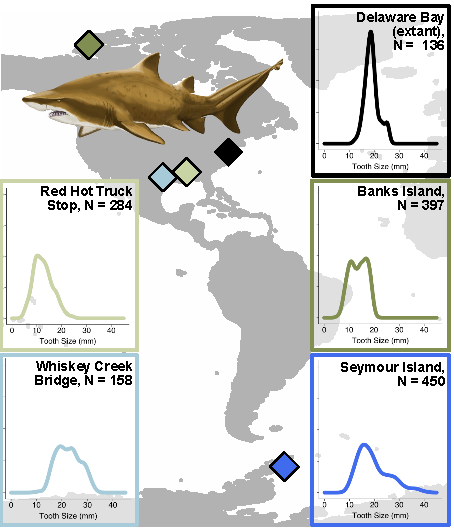
\includegraphics[width=0.5\linewidth]{Shark_Map4C.pdf}
    \caption{Map of sand tiger shark localities and their size distributions. Extant sand tiger sharks were caught at a mid-latitude marine site, Delaware Bay (black), where total length was measured and transformed to anterior tooth crown height.  Eocene site size distributions are based on anterior tooth crown measurements. During the Eocene, the extinct \emph{Striatolamia macrota} inhabited both high latitude waters (darker shades), such as Banks Island in the Canadian Arctic (Eureka Sound Fm., dark green), Seymour Island off the Antarctic Peninsula (La Meseta Fm., dark blue) and mid-latitude waters (lighter shades) in the Gulf of Mexico, such as the Red Hot Truck Stop in Mississippi (Bashi/Tuscahoma Fm., light green) and Whiskey Bridge in Texas (Crockett Fm., light blue). In addition to paired latitude, these sites were also chosen to represent brackish  (Banks Island, high latitude, and Red Hot Truck Stop, low latitude; greens) and marine  (Seymour Island, high latitude, and Whiskey Bridge, low latitude; blues) waters. ${}^\dag$\emph{Striatolamia macrota} illustration by Christina Spence Morgan.}
\label{fig:map}
\end{figure}

\begin{figure}[ht]
  \centering
  % include first image
  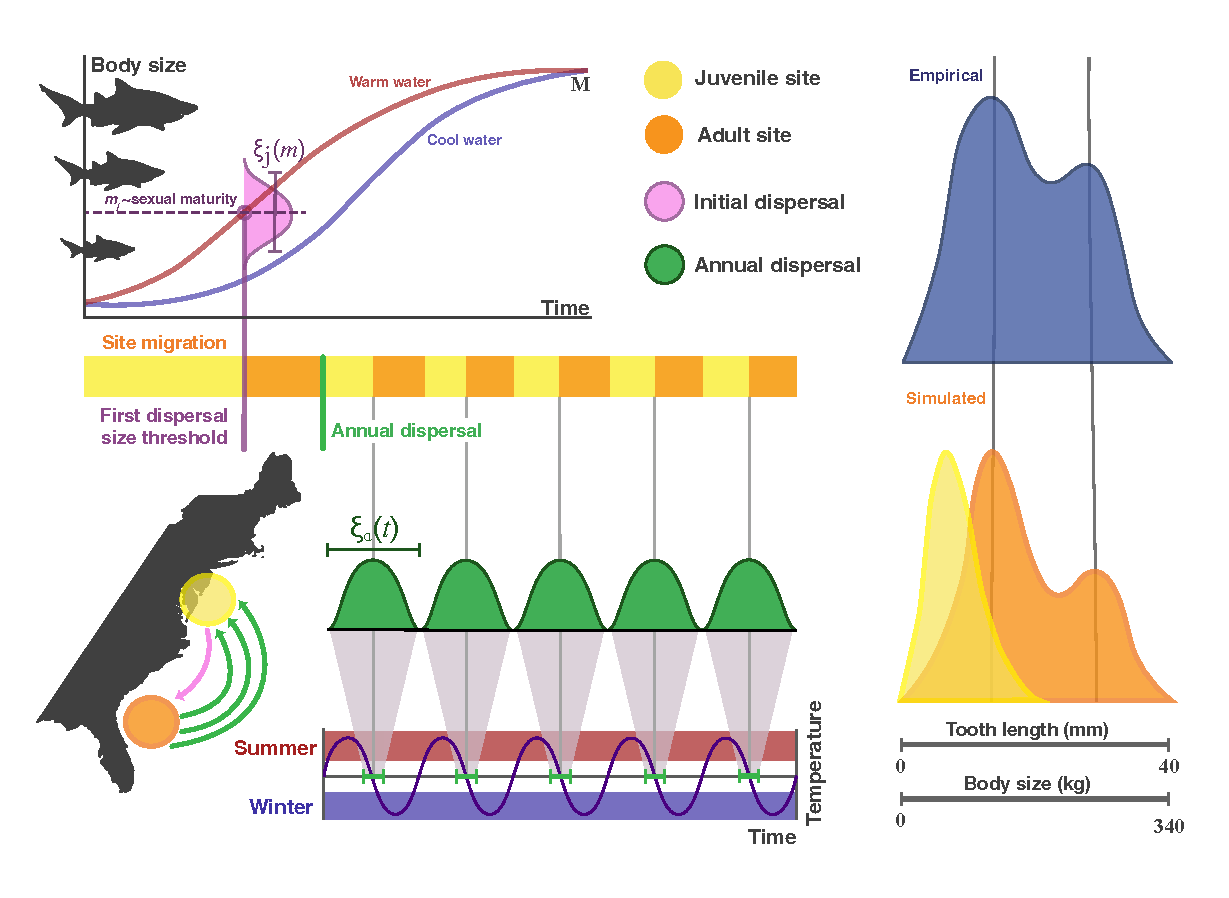
\includegraphics[width=1\linewidth]{BodySizeFigure_Draft2_Jan6.pdf}  
   \caption{Conceptual diagram of the population simulation where sand tiger shark individuals migrate between a juvenile site or nursery (yellow) and adult site (orange). 
   The ontogenetic growth rates of sand tiger individuals increase with temperature (blue and red growth curves) from an initial mass $m_0$ to an asymptotic mass $M$.
   After birth, newborns reside in the juvenile site until they reach maturity at mass $m_j$, after which they disperse to the adult site.
   The juvenile dispersal window $\xi_j$ (pink) denotes the variability in size at which initial dispersal occurs. 
   Adults disperse to the juvenile site, where $\xi_a$ denotes the variability in the timing of the migration (green), which occurs annually from the adult to the juvenile site and back (map inset).
   Individuals drop teeth as they migrate, such that accumulating dental distributions capture the size structure of populations at both sites.
   Empirical dental distributions (blue distribution) can be compared to simulated distributions at juvenile and adult sites (yellow and orange distributions, respectively) and evaluated for best-fit based on mean, variance, and modality, thereby gaining insight into life-history characteristics such as the juvenile and adult dispersal windows. Illustration by Christina Spence Morgan.}
  \label{fig:diagram}
\end{figure}

\begin{figure}[ht]
  \centering
  % include first image
  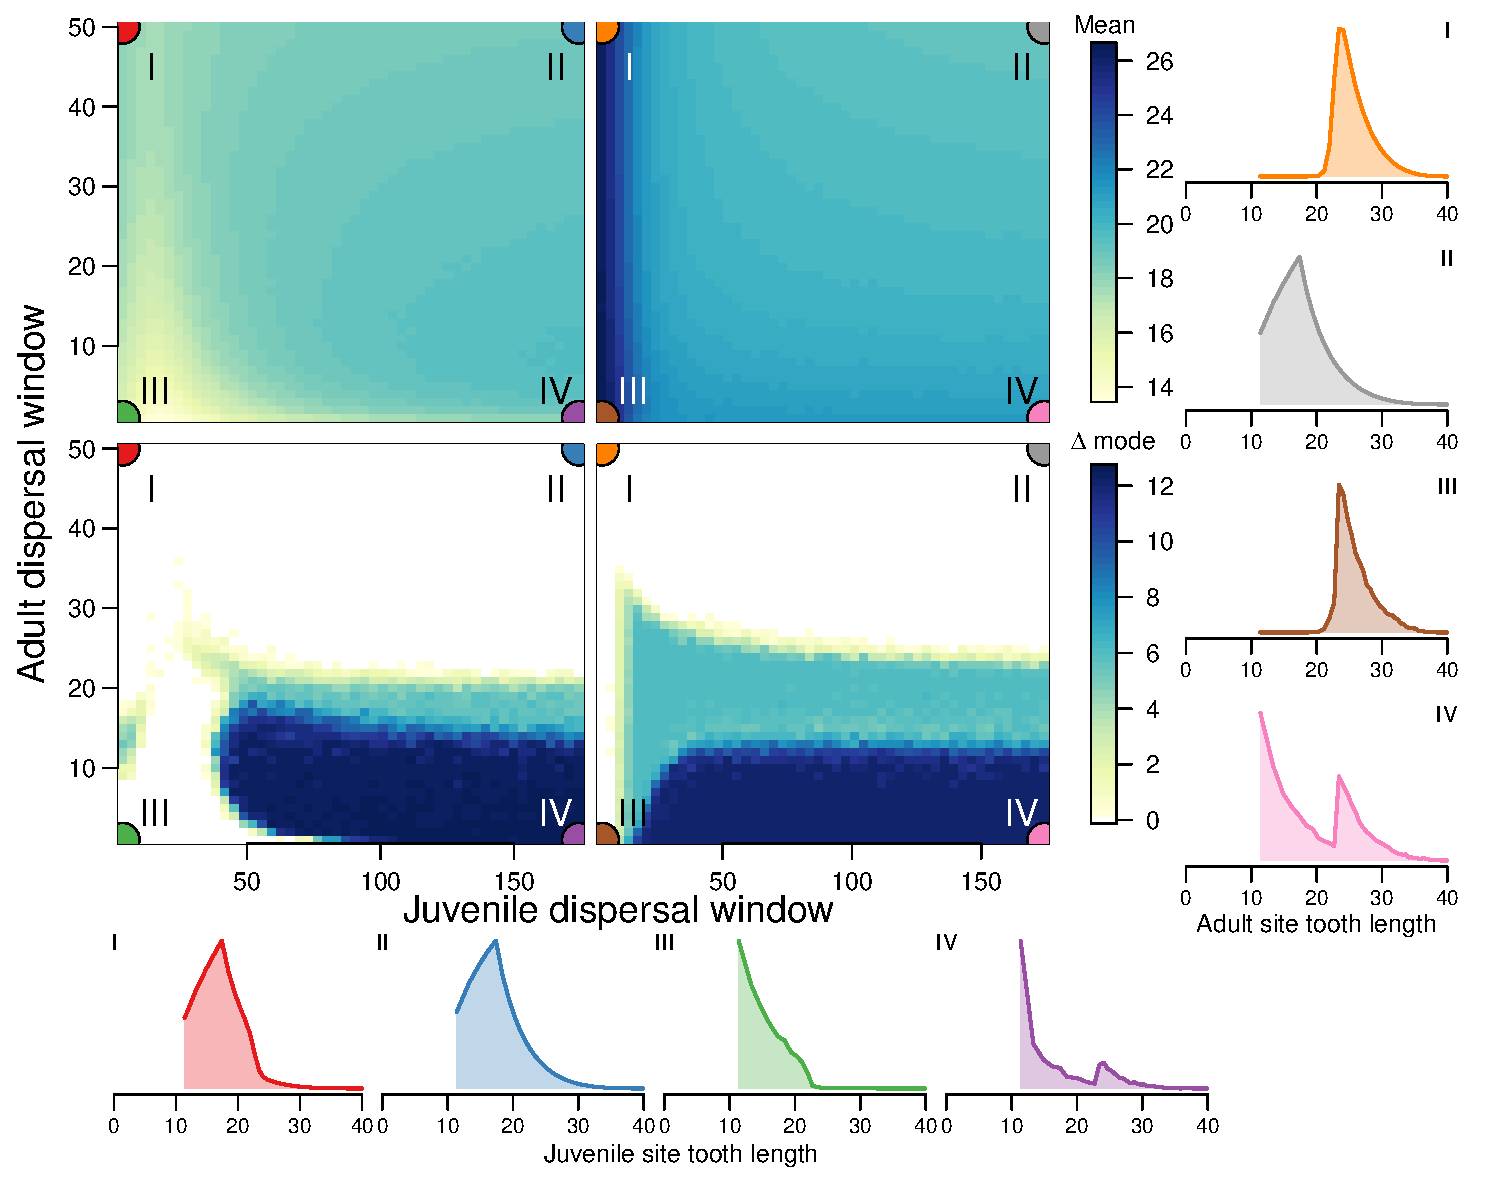
\includegraphics[width=1\linewidth]{fig_means_peaks_highlatitude_rev.pdf}  
%   \caption{}
%   \label{fig:sub-first}

\caption{Simulation results for the dynamic population model as a function of juvenile and adult dispersal windows ($\xi_j$ and $\xi_a$, respectively). 
Changes in dental distribution shape are captured by site-specific means (top two panels) and the distance between modes ($\Delta$ mode; bottom two panels).
A $\Delta$ mode value of zero means there is only one mode.
Representative distributions of anterior tooth crown height are shown for juvenile site and adult sites for regions I-IV  (horizontal along bottom and vertical along right edge, respectively), where color denotes both region and site identity.
Regions I-IV depict various combinations of small and large dispersal windows. Region I (high $\xi_a$, low $\xi_j$); II (high $\xi_a$, high $\xi_j$); III (low $\xi_a$, low $\xi_j$); IV (low $\xi_a$, high $\xi_j$).
Results are shown for high altitude Eocene conditions, but are qualitatively similar for all evaluated localities.
% Note the multiple modes that arise when juveniles can leave the nursery across a large body size gradient and adult migration is tightly constrained, as in region IV with size structure for juvenile and adult sites in purple and pink distributions in bottom right.
}
\label{fig:sim}
\end{figure}

\begin{figure}[ht]
  \centering
  % include first image
  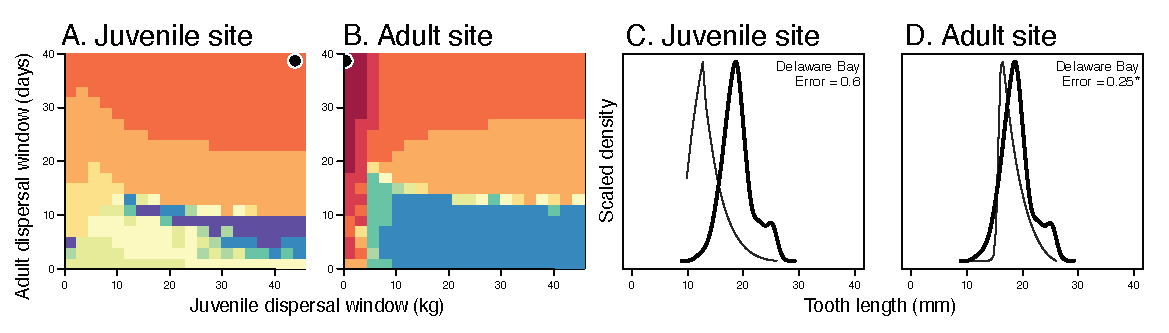
\includegraphics[width=1\linewidth]{fig_empirical_comp_Delaware2.pdf}  
%   \caption{}
%   \label{fig:sub-first}

\caption{Comparison of empirical dental distributions from sand tigers in the Delaware Bay and those simulated across different values of the juvenile ($\xi_j$) and adult ($\xi_a$) dispersal windows.
Better fits between empirical and simulated distributions at juvenile (A) and adult sites (B) are represented by warmer colors (lower $\epsilon$; Eq. \ref{eq:error}). 
Best-fit simulation results for juvenile and adult simulation results at a particular $(\xi_j,\xi_a)$ are denoted by black circles.
The corresponding distributions at this best-fit value of $(\xi_j,\xi_a)$ are shown for juvenile (C) and adult (D) sites for comparison (thin lines) relative to the empirical distribution (thick line). 
Within-site best-fit error values are reported in the upper-right, and the across-site best-fit error is denoted with an asterisk (${}^\ast$).
% The empirical-simulation comparison (empirical = bold black line, simulation = thin black line; error shown in top right) suggests the Delaware Bay is an adult site, which is consistent with modern ecological studies \cite{Teter2015, heupel2014sizing}.
}
\label{fig:compmodern}
\end{figure}




% \usepackage{subcaption}
\begin{figure}[ht]

  \centering
  % include first image
  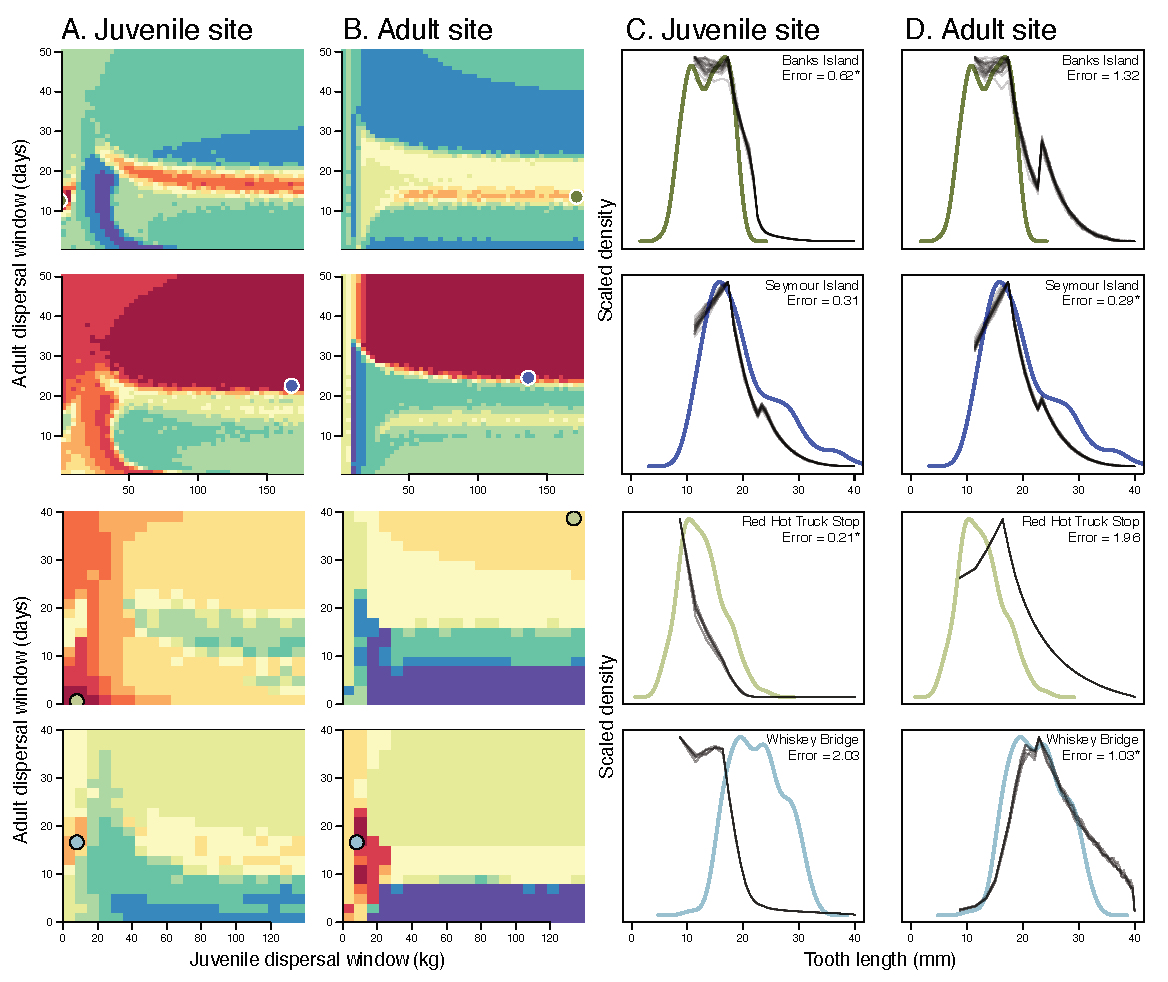
\includegraphics[width=1\linewidth]{fig_empirical_eocene_comp_all2.pdf}  
%   \caption{}
%   \label{fig:sub-first}

\caption{
% A comparison of Eocene empirical results and simulation fit for juvenile (A) and adult sites (B) for a range of migration windows. Each pixel represents the fit of simulation results to empirical data, with best fit in warmer colors. The top two rows are high latitude sites, Banks Island (dark green) and Seymour Island (dark blue), while bottom two rows are mid-latitude sites, Red Hot Truck Stop (light green) and Whiskey Bridge (light blue). The best fit juvenile and adult migration windows for  the juvenile and adult sites are shown as a circle corresponding to the site colors (A, B) and anterior tooth crown height distributions for the simulation (black lines) and empirical (color line) data are shown for comparison (C, D). Based on the lower error (shown in top right of each panel), we hypothesize each locality as a juvenile or adult site, as indicated with "*". The only site we were not able to confidently resolve is Seymour Island. 
Comparison of empirical dental distributions from sand tigers at Eocene localities and those simulated across different values of the juvenile ($\xi_j$) and adult ($\xi_a$) dispersal windows.
Eocene localities include the high latitude Banks Island (first row, dark green) and Seymour Island (second row, dark blue) sites as well as the low latitude Red Hot Truck Stop (third row, light green) and Whiskey Bridge Sites (fourth row, light blue).
Blues denote sites reconstructed as marine habitats; greens denote sites reconstructed as near-shore estuarine habitats.
Across all rows, better fits between empirical and simulated distributions at juvenile (A) and adult sites (B) are represented by warmer colors (lower $\epsilon$; Eq. \ref{eq:error}). 
Best-fit simulation results for juvenile and adult simulation results at a particular $(\xi_j,\xi_a)$ are denoted by colored circles.
The corresponding distributions at this best-fit value of $(\xi_j,\xi_a)$ are shown for juvenile (C) and adult (D) sites for comparison (thin lines) relative to the empirical distribution (thick line). 
Within-site best-fit error values are reported in the upper-right, and the across-site best-fit error is denoted with an asterisk (${}^\ast$).}
\label{fig:comp}
\end{figure}


\clearpage
%%%%%%%%%% Insert bibliography here %%%%%%%%%%%%%%
% \bibliographystyle{RS}
% \bibliography{aa_starving3}

\begin{thebibliography}{99}

\bibitem{sibert2018two}
Sibert E, Friedman M, Hull P, Hunt G, Norris R. 2018  Two pulses of
  morphological diversification in Pacific pelagic fishes following the
  Cretaceous--Palaeogene mass extinction. {\em Proceedings of the Royal Society
  B} \textbf{285}, 20181194.

\bibitem{sibert2021early}
Sibert EC, Rubin LD. 2021  An early Miocene extinction in pelagic sharks. {\em
  Science} \textbf{372}, 1105--1107.

\bibitem{naylor2021comment}
Naylor GJ, de~Lima A, Castro JI, Hubbell G, de~Pinna MC. 2021  Comment on “An
  early Miocene extinction in pelagic sharks”. {\em Science} \textbf{374},
  eabj8723.

\bibitem{feichtinger2021comment}
Feichtinger I, Adnet S, Cuny G, Guinot G, Kriwet J, Neubauer T, Pollersp{\"o}ck
  J, Shimada K, Straube N, Underwood C et~al.. 2021  Comment on “An early
  Miocene extinction in pelagic sharks”. {\em Science} \textbf{374},
  eabk0632.

\bibitem{Shimada2002}
Shimada K. 2002  {Dental homologies in lamniform sharks (Chondrichthyes:
  Elasmobranchii)}. {\em Journal of Morphology} \textbf{251}, 38--72.

\bibitem{Shimada2004}
Shimada K. 2004  {The relationship between the tooth size and total body length
  in the sandtiger shark, Carcharias taurus (Laminformes : Odontaspidae)}. {\em
  Journal of Fossil Research} \textbf{37}, 76--81.

\bibitem{Shimada2007}
Shimada K. 2007  {Skeletal and dental anatomy of lamniform shark, Cretalamna
  appendiculata, from Upper Cretaceous Niobrara Chalk of Kansas}. {\em Journal
  of Vertebrate Paleontology} \textbf{27}, 584--602.

\bibitem{Kim2014d}
Kim SSL, Eberle JJJ, Bell DDM, Fox DDA, Padilla A. 2014  {Evidence from shark
  teeth for a brackish Arctic Ocean in the Eocene greenhouse}. {\em Geology}
  \textbf{42}, 695--698.

\bibitem{zacke2009surface}
Zacke A, Voigt S, Joachimski MM, Gale AS, Ward DJ, T{\"u}tken T. 2009
  Surface-water freshening and high-latitude river discharge in the Eocene
  North Sea. {\em Journal of the Geological Society} \textbf{166}, 969--980.

\bibitem{Kim2020}
Kim SL, Zeichner SS, Colman AS, Scher HD, Kriwet J, M{\"{o}}rs T, Huber M. 2020
   { Probing the ecology and climate of the Eocene Southern Ocean with sand
  tiger sharks Striatolamia macrota }. {\em Paleoceanography and
  Paleoclimatology} pp. 1--21.

\bibitem{straube2020intraspecific}
Straube N, Pollersp{\"o}ck J. 2020  Intraspecific dental variations in the
  deep-sea shark Etmopterus spinax and their significance in the fossil record.
  {\em Zoomorphology} \textbf{139}, 483--491.

\bibitem{Pimiento2010}
Pimiento C, Ehret DJ, MacFadden BJ, Hubbell G. 2010  {Ancient nursery area for
  the extinct giant shark megalodon from the Miocene of Panama}. {\em PLoS ONE}
  \textbf{5}.

\bibitem{herraiz2020use}
Herraiz JL, Rib{\'e} J, Botella H, Mart{\'\i}nez-P{\'e}rez C, Ferr{\'o}n HG.
  2020  Use of nursery areas by the extinct megatooth shark Otodus megalodon
  (Chondrichthyes: Lamniformes). {\em Biology letters} \textbf{16}, 20200746.

\bibitem{Villafana2020}
Villafa{\~{n}}a JA, Hernandez S, Alvarado A, Shimada K, Pimiento C, Rivadeneira
  MM, Kriwet J. 2020  {First evidence of a palaeo-nursery area of the great
  white shark}. {\em Scientific Reports} \textbf{10}, 1--8.

\bibitem{brose2006consumer}
Brose U, Jonsson T, Berlow EL, Warren P, Banasek-Richter C, Bersier LF,
  Blanchard JL, Brey T, Carpenter SR, Blandenier MFC et~al.. 2006
  Consumer--resource body-size relationships in natural food webs. {\em
  Ecology} \textbf{87}, 2411--2417.

\bibitem{West:2001bv}
West GB, Brown JH, Enquist BJ. 2001  {A general model for ontogenetic growth}.
  {\em Nature} \textbf{413}, 628--631.

\bibitem{bhat2020scaling}
Bhat U, Kempes CP, Yeakel JD. 2020  Scaling the risk landscape drives optimal
  life-history strategies and the evolution of grazing. {\em Proceedings of the
  National Academy of Sciences} \textbf{117}, 1580--1586.

\bibitem{schindler2002sharks}
Schindler DE, Essington TE, Kitchell JF, Boggs C, Hilborn R. 2002  Sharks and
  tunas: fisheries impacts on predators with contrasting life histories. {\em
  Ecological Applications} \textbf{12}, 735--748.

\bibitem{heithaus2007nursery}
Heithaus MR. 2007  Nursery areas as essential shark habitats: a theoretical
  perspective. In {\em American Fisheries Society Symposium} vol.~50 p.~3.
  American Fisheries Society.

\bibitem{doan2020adult}
Doan MD, Kajiura SM. 2020  Adult blacktip sharks (Carcharhinus limbatus) use
  shallow water as a refuge from great hammerheads (Sphyrna mokarran). {\em
  Journal of fish biology} \textbf{96}, 1530--1533.

\bibitem{heupel2007shark}
Heupel MR, Carlson JK, Simpfendorfer CA. 2007  Shark nursery areas: concepts,
  definition, characterization and assumptions. {\em Marine Ecology Progress
  Series} \textbf{337}, 287--297.

\bibitem{burke2018pliocene}
Burke KD, Williams JW, Chandler MA, Haywood AM, Lunt DJ, Otto-Bliesner BL. 2018
   Pliocene and Eocene provide best analogs for near-future climates. {\em
  Proceedings of the National Academy of Sciences} \textbf{115}, 13288--13293.

\bibitem{Waddell2008}
Waddell LM, Moore TC. 2008  {Salinity of the Eocene Arctic Ocean from oxygen
  isotope analysis of fish bone carbonate}. {\em Paleoceanography} \textbf{23},
  1--14.

\bibitem{greenwood2010wet}
Greenwood DR, Basinger JF, Smith RY. 2010  How wet was the Arctic Eocene rain
  forest? Estimates of precipitation from Paleogene Arctic macrofloras. {\em
  Geology} \textbf{38}, 15--18.

\bibitem{padilla2014sand}
Padilla A, Eberle JJ, Gottfried MD, Sweet AR, Hutchison JH. 2014  A sand tiger
  shark--dominated fauna from the Eocene Arctic greenhouse. {\em Journal of
  Vertebrate Paleontology} \textbf{34}, 1307--1316.

\bibitem{Ivany2008}
Ivany LC, Lohmann KC, Hasiuk F, Blake DB, Glass A, Aronson RB, Moody RM. 2008
  {Eocene climate record of a high southern latitude continental shelf: Seymour
  Island, Antarctica}. {\em Bulletin of the Geological Society of America}
  \textbf{120}, 659--678.

\bibitem{Long1992}
Long DJ. 1992  {Sharks from the La Meseta Formation (Eocene), Seymour Island,
  Antarctic Peninsula}. {\em Journal of Vertebrate Paleontology} \textbf{12},
  11--32.

\bibitem{Kriwet2016}
Kriwet J, Engelbrecht A, M{\"{o}}rs T, Reguero M, Pfaff C. 2016  {Ultimate
  Eocene (Priabonian) chondrichthyans (Holocephali, Elasmobranchii) of
  Antarctica}. {\em Journal of Vertebrate Paleontology} \textbf{36}.

\bibitem{Kriwet2005}
Kriwet J. 2005  {Additions to the Eocene selachian fauna of Antarctica with
  comments on Antarctic selachian diversity}. {\em Journal of Vertebrate
  Paleontology} \textbf{25}, 1--7.

\bibitem{Reguero2012}
Reguero MA, Marenssi SA, Santillana SN. 2012  {Weddellian marine/coastal
  vertebrates diversity from a basal horizon (Ypresian, Eocene) of the
  Cucullaea I Allomember, La Meseta formation, Seymour (Marambio) Island,
  Antarctica}. {\em Rev. peru. biol.} \textbf{19}, 275--284.

\bibitem{Engelbrecht2019}
Engelbrecht A, M{\"{o}}rs T, Reguero MA, Kriwet J. 2019  {Skates and rays
  (Elasmobranchii, Batomorphii) from the Eocene La Meseta and Submeseta
  formations, Seymour Island, Antarctica}. {\em Historical Biology}
  \textbf{31}, 1028--1044.

\bibitem{Padilla2014}
Padilla A, Eberle JJ, Gottfried MD, Sweet AR, Hutchison JH. 2014  {A sand tiger
  shark-dominated fauna from the Eocene Arctic greenhouse}. {\em Journal of
  Vertebrate Paleontology} \textbf{34}, 1307--1316.

\bibitem{purdy1998chondrichthyan}
Purdy RW. 1998  Chondrichthyan fishes from the Paleocene of South Carolina.
  {\em Transactions of the American philosophical society} pp. 122--146.

\bibitem{Westgate}
Westgate JW. 2001  Paleoecology and biostratigraphy of marginal marine Gulf
  Coast Eocene vertebrate localities. In {\em Eocene biodiversity} ,  pp.
  263--297. Springer.

\bibitem{ingram1991tuscahoma}
Ingram S. 1991  The Tuscahoma-Bashi section at Meridian, Mississippi: First
  notice of lowstand deposits above the Paleocene--Eocene TP2/TE1 sequence
  boundary. {\em Mississippi Geology} \textbf{11}, 9--14.

\bibitem{Beard2009}
Beard KC, Dawson MR. 2009  Early Wasatchian mammals of the red hot local fauna,
  uppermost Tuscahoma formation, Lauderdale County, Mississippi. {\em Annals of
  Carnegie Museum} \textbf{78}, 193--243.

\bibitem{Breard1999}
Breard SQ, Stringer GL. 1999  {Abstract: Integrated Paleoecology and Marine
  Vertebrate Fauna of the Stone City Formation (Middle Eocene), Brazos River
  Section, Texas }. {\em AAPG Bulletin} \textbf{83}.

\bibitem{harding2014mineralogy}
Harding SC, Nash BP, Petersen EU, Ekdale A, Bradbury CD, Dyar MD. 2014
  Mineralogy and geochemistry of the Main Glauconite Bed in the Middle Eocene
  of Texas: Paleoenvironmental implications for the Verdine Facies. {\em PloS
  one} \textbf{9}, e87656.

\bibitem{Jorgensen2010}
Jorgensen SJ, Reeb CA, Chapple TK, Anderson S, Perle C, {Van Sommeran} SR,
  Fritz-Cope C, Brown AC, Klimley AP, Block BA. 2010  {Philopatry and migration
  of Pacific white sharks}. {\em Proceedings of the Royal Society B: Biological
  Sciences} \textbf{277}, 679--688.

\bibitem{Macdonald2021}
Macdonald C, Perni N, Jerome J, Wester J, Black K, Shiffman D. 2021  {First
  identification of probable nursery habitat for critically endangered great
  hammerhead Sphyrna mokarran on the Atlantic Coast of the United States}. {\em
  Conservation Science and Practice} \textbf{3}, 1--6.

\bibitem{Cappetta2012}
Cappetta H. 2012 {\em {Handbook of Paleoichthyology, Volume 3E}}.
Munich: Verlag chondricht edition.

\bibitem{Cunningham2000}
Cunningham SB. 2000  {A comparison of isolated teeth of early Eocene
  Striatolamia macrota (Chondrichthyes , Lamniformes), with those of a Recent
  sand shark , Carcharias taurus}. {\em Tertiary Research} \textbf{20}, 17--31.

\bibitem{haulsee2016implantation}
Haulsee DE, Fox DA, Breece MW, Clauss TM, Oliver MJ. 2016  Implantation and
  recovery of long-term archival transceivers in a migratory shark with high
  site fidelity. {\em PloS one} \textbf{11}, e0148617.

\bibitem{haulsee2018spatial}
Haulsee D, Breece M, Brown L, Wetherbee B, Fox D, Oliver M. 2018  Spatial
  ecology of Carcharias taurus in the northwestern Mid-Atlantic coastal ocean.
  {\em Marine Ecology Progress Series} \textbf{597}, 191--206.

\bibitem{Teter2015}
Teter SM, Wetherbee BM, Fox DA, Lam CH, Kiefer DA, Shivji M. 2015  {Migratory
  patterns and habitat use of the sand tiger shark (Carcharias taurus) in the
  western North Atlantic}. {\em Marine and Freshwater Research} \textbf{66},
  158--169.

\bibitem{kilfoil2017targeted}
Kilfoil JP, Wetherbee BM, Carlson JK, Fox DA. 2017  Targeted catch-and-release
  of prohibited sharks: sand tigers in coastal Delaware waters. {\em Fisheries}
  \textbf{42}, 281--287.

\bibitem{Kneebone2012}
Kneebone J, Chisholm J, Skomal GB. 2012  {Seasonal residency, habitat use, and
  site fidelity of juvenile sand tiger sharks Carcharias taurus in a
  Massachusetts estuary}. {\em Marine Ecology Progress Series} \textbf{471},
  165--181.

\bibitem{Goldman2006}
Goldman KJ, Branstetter S, Musick JA. 2006  {A re-examination of the age and
  growth of sand tiger sharks, Carcharias taurus, in the western North
  Atlantic: The importance of ageing protocols and use of multiple
  back-calculation techniques}. {\em Environmental Biology of Fishes}
  \textbf{77}, 241--252.

\bibitem{cortes1996comparative}
Cort{\'e}s E, Parsons GR. 1996  Comparative demography of two populations of
  the bonnethead shark (Sphyrna tiburo). {\em Canadian Journal of Fisheries and
  Aquatic Sciences} \textbf{53}, 709--718.

\bibitem{moses2008rmo}
Moses ME, Hou C, Woodruff WH, West GB, Nekola JC, Zuo W, Brown JH. 2008
  {Revisiting a Model of Ontogenetic Growth: Estimating Model Parameters from
  Theory and Data}. {\em http://dx.doi.org.proxy.lib.sfu.ca/10.1086/679735}
  \textbf{171}, 632--645.

\bibitem{gillooly2002esa}
Gillooly JF, Charnov EL, West GB, Savage VM, Brown JH. 2002  {Effects of size
  and temperature on developmental time}. {\em Nature} \textbf{417}, 70--73.

\bibitem{hou}
Hou C, Zuo W, Moses ME, Woodruff WH, Brown JH, West GB. 2008  {Energy Uptake
  and Allocation During Ontogeny}. {\em Science} \textbf{322}, 736--739.

\bibitem{Kempes:2012hy}
Kempes CP, Dutkiewicz S, Follows MJ. 2012  {Growth, metabolic partitioning, and
  the size of microorganisms.}. {\em PNAS} \textbf{109}, 495--500.

\bibitem{Pirt1965}
Pirt S. 1965  {The maintenance energy of bacteria in growing cultures}. {\em
  Proc. Roy. Soc. B} \textbf{163}, 224.

\bibitem{Heijnen1981}
Heijnen JJ, Roels JA. 1981  {A macroscopic model describing yield and
  maintenance relationships in aerobic fermentation processes}. {\em
  Biotechnology and Bioengineering} \textbf{23}, 739--763.

\bibitem{yeakel2018dynamics}
Yeakel JD, Kempes CP, Redner S. 2018  Dynamics of starvation and recovery
  predict extinction risk and both Damuth’s law and Cope’s rule. {\em
  Nature communications} \textbf{9}, 1--10.

\bibitem{Brown2004}
Brown JH, Gillooly JF, Allen AP, Savage VM, West GB. 2004  {Toward a metabolic
  theory of ecology}. {\em Ecology} \textbf{85}, 1771--1789.

\bibitem{zeichner2017discrimination}
Zeichner S, Colman A, Koch P, Polo-Silva C, Galv{\'a}n-Maga{\~n}a F, Kim S.
  2017  Discrimination factors and incorporation rates for organic matrix in
  shark teeth based on a captive feeding study. {\em Physiological and
  Biochemical Zoology} \textbf{90}, 257--272.

\bibitem{cantrill2012vegetation}
Cantrill DJ, Poole I. 2012 {\em The vegetation of Antarctica through geological
  time}.
Cambridge University Press.

\bibitem{miall1986eureka}
Miall AD. 1986  The Eureka Sound Group (Upper Cretaceous-Oligocene), Canadian
  Arctic Islands. {\em Bulletin of Canadian Petroleum Geology} \textbf{34},
  240--270.

\bibitem{eberle2012life}
Eberle JJ, Greenwood DR. 2012  Life at the top of the greenhouse Eocene
  world—A review of the Eocene flora and vertebrate fauna from Canada’s
  High Arctic. {\em Bulletin} \textbf{124}, 3--23.

\bibitem{marenssi2002provenance}
Marenssi SA, Net LI, Santillana SN. 2002  Provenance, environmental and
  paleogeographic controls on sandstone composition in an incised-valley
  system: the Eocene La Meseta Formation, Seymour Island, Antarctica. {\em
  Sedimentary Geology} \textbf{150}, 301--321.

\bibitem{beard2008oldest}
Beard KC. 2008  The oldest North American primate and mammalian biogeography
  during the Paleocene--Eocene Thermal Maximum. {\em Proceedings of the
  National Academy of Sciences} \textbf{105}, 3815--3818.

\bibitem{Flis2017}
Flis JE, Yancey TE, Flis CJ. 2017  {Middle Eocene Storm Deposition in the
  Northwestern Gulf of Mexico, Burleson County, Texas, U.S.A}. {\em Gulf Coast
  Association of Geological Societies} \textbf{6}, 201--225.

\bibitem{heupel2014sizing}
Heupel MR, Knip DM, Simpfendorfer CA, Dulvy NK. 2014  Sizing up the ecological
  role of sharks as predators. {\em Marine Ecology Progress Series}
  \textbf{495}, 291--298.

\bibitem{kneebone2014movement}
Kneebone J, Chisholm J, Skomal G. 2014  Movement patterns of juvenile sand
  tigers (Carcharias taurus) along the east coast of the USA. {\em Marine
  Biology} \textbf{161}, 1149--1163.

\bibitem{otway2011pop}
Otway N, Ellis M. 2011  Pop-up archival satellite tagging of Carcharias taurus:
  movements and depth/temperature-related use of south-eastern Australian
  waters. {\em Marine and Freshwater Research} \textbf{62}, 607--620.

\bibitem{sluijs2008arctic}
Sluijs A, R{\"o}hl U, Schouten S, Brumsack HJ, Sangiorgi F, Damst{\'e} JSS,
  Brinkhuis H. 2008  Arctic late Paleocene--early Eocene paleoenvironments with
  special emphasis on the Paleocene-Eocene thermal maximum (Lomonosov Ridge,
  Integrated Ocean Drilling Program Expedition 302). {\em Paleoceanography}
  \textbf{23}.

\bibitem{eberle2010seasonal}
Eberle JJ, Fricke HC, Humphrey JD, Hackett L, Newbrey MG, Hutchison JH. 2010
  Seasonal variability in Arctic temperatures during early Eocene time. {\em
  Earth and Planetary Science Letters} \textbf{296}, 481--486.

\bibitem{west2015arctic}
West CK, Greenwood DR, Basinger JF. 2015  Was the Arctic Eocene
  ‘rainforest’monsoonal? Estimates of seasonal precipitation from early
  Eocene megafloras from Ellesmere Island, Nunavut. {\em Earth and Planetary
  Science Letters} \textbf{427}, 18--30.

\bibitem{west2020paleobotanical}
West CK, Greenwood DR, Reichgelt T, Lowe AJ, Vachon JM, Basinger JF. 2020
  Paleobotanical proxies for early Eocene climates and ecosystems in northern
  North America from middle to high latitudes. {\em Climate of the Past}
  \textbf{16}, 1387--1410.

\bibitem{zhu2020simulation}
Zhu J, Poulsen CJ, Otto-Bliesner BL, Liu Z, Brady EC, Noone DC. 2020
  Simulation of early Eocene water isotopes using an Earth system model and its
  implication for past climate reconstruction. {\em Earth and Planetary Science
  Letters} \textbf{537}, 116164.

\bibitem{keating2011warm}
Keating-Bitonti CR, Ivany LC, Affek HP, Douglas P, Samson SD. 2011  Warm, not
  super-hot, temperatures in the early Eocene subtropics. {\em Geology}
  \textbf{39}, 771--774.

\bibitem{ivany2004intra}
Ivany LC, Wilkinson BH, Lohmann KC, Johnson ER, McElroy BJ, Cohen GJ. 2004
  Intra-annual isotopic variation in Venericardia bivalves: implications for
  early Eocene temperature, seasonality, and salinity on the US Gulf Coast.
  {\em Journal of Sedimentary Research} \textbf{74}, 7--19.

\bibitem{Hopkins1974}
Hopkins W. 1974  Report on 36 Field Samples from Banks Island, District of
  Franklin, Northwest Territories, Submitted by A. Miall, 1973 (NTS 88C, F,
  98D, E), Geological Survey of Canada. Technical report Paleontological Report
  KT-01-WSH-1974.

\bibitem{Hopkins1975}
Hopkins W. 1975  Palynology Report on 44 Field Samples from Banks Island,
  Submitted by AD Miall, 1974 (NTS 88B, C, F, 97H, 98D, E); Geological Survey
  of Canada. Technical report Paleontological Report KT-10-WSH-1975.

\bibitem{Miall1979}
Miall AD. 1979  {Mesozoic and Tertiary geology of Banks Island, Arctic Canada:
  the history of an unstable craton margin}. {\em Geological Survey of Canada
  Memoir} \textbf{387}, 1--235.

\bibitem{Sweet2012}
Sweet A. 2012  Applied research report on 5 outcrop samples collected by Andrew
  Miall from northern Banks Island. {\em NWT (NTS Map Sheets 098E/01, 08, 09):
  Geological Survey of Canada Paleontological report ARS-2012-01}.

\bibitem{eberle2014first}
Eberle JJ, Gottfried MD, Hutchison JH, Brochu CA. 2014  First record of Eocene
  bony fishes and crocodyliforms from Canada’s Western Arctic. {\em PloS one}
  \textbf{9}, e96079.

\bibitem{Stilwell1992}
Stilwell JD, Zinsmeister WJ. 1992 {\em {Molluscan systematics and
  biostratigraphy: Lower Tertiary La Meseta Formation, Seymour Island,
  Antarctic Peninsula}}.
Washington: American Geophysical Union antarctic edition.

\bibitem{Marenssi1994}
Marenssi SA, Reguero MA, Santillana SN, Vizcaino SF. 1994  {Review Eocene land
  mammals from Seymour Island, Antarctica: palaeobiogeographical implications}.
  .

\bibitem{Amenabar2020}
Amen{\'{a}}bar CR, Montes M, Nozal F, Santillana S. 2020  {Dinoflagellate cysts
  of the la Meseta Formation (middle to late Eocene), Antarctic Peninsula:
  Implications for biostratigraphy, palaeoceanography and palaeoenvironment}.
  {\em Geological Magazine} \textbf{157}, 351--366.

\bibitem{douglas2014pronounced}
Douglas PM, Affek HP, Ivany LC, Houben AJ, Sijp WP, Sluijs A, Schouten S,
  Pagani M. 2014  Pronounced zonal heterogeneity in Eocene southern
  high-latitude sea surface temperatures. {\em Proceedings of the National
  Academy of Sciences} \textbf{111}, 6582--6587.

\bibitem{eagles2006small}
Eagles G, Livermore R, Morris P. 2006  Small basins in the Scotia Sea: the
  Eocene Drake passage gateway. {\em Earth and Planetary Science Letters}
  \textbf{242}, 343--353.

\bibitem{scher2006timing}
Scher HD, Martin EE. 2006  Timing and climatic consequences of the opening of
  Drake Passage. {\em science} \textbf{312}, 428--430.

\bibitem{Harrington2003}
Harrington GJ. 2003  {Wasatchian (Early Eocene) pollen floras from the Red Hot
  Truck Stop, Mississippi, USA}. {\em Palaeontology} \textbf{46}, 725--738.

\bibitem{basinger1994early}
Basinger J, Greenwood D, Sweda T. 1994  Early Tertiary vegetation of Arctic
  Canada and its relevance to paleoclimatic interpretation. In {\em Cenozoic
  plants and climates of the Arctic} ,  pp. 175--198. Springer.

\bibitem{sluijs2009warm}
Sluijs A, Schouten S, Donders TH, Schoon PL, R{\"o}hl U, Reichart GJ, Sangiorgi
  F, Kim JH, Damst{\'e} JSS, Brinkhuis H. 2009  Warm and wet conditions in the
  Arctic region during Eocene Thermal Maximum 2. {\em Nature Geoscience}
  \textbf{2}, 777--780.

\bibitem{kobashi2003oxygen}
Kobashi T, Grossman EL. 2003  The oxygen isotopic record of seasonality in
  Conus shells and its application to understanding late middle Eocene (38 Ma)
  climate. {\em Paleontological Research} \textbf{7}, 343--355.

\bibitem{montes2019late}
Montes M, Beamud E, Nozal F, Santillana S. 2019  Late Maastrichtian-Paleocene
  chronostratigraphy from Seymour Island (James Ross Basin, Antarctic
  Peninsula). Eustatic controls of sedimentation. {\em Advances in Polar
  Science} \textbf{30}, 303--327.

\bibitem{jorgensen2012eating}
Jorgensen SJ, Arnoldi NS, Estess EE, Chapple TK, R{\"u}ckert M, Anderson SD,
  Block BA. 2012  Eating or meeting? Cluster analysis reveals intricacies of
  white shark (Carcharodon carcharias) migration and offshore behavior. {\em
  PloS one} \textbf{7}, e47819.

\bibitem{dicken2008estimates}
Dicken ML, Booth AJ, Smale MJ. 2008  Estimates of juvenile and adult
  raggedtooth shark (Carcharias taurus) abundance along the east coast of South
  Africa. {\em Canadian Journal of Fisheries and Aquatic Sciences} \textbf{65},
  621--632.

\bibitem{castro1987position}
Castro JI. 1987  The position of sharks in marine biological communities: an
  overview. {\em Sharks, An Inquiry into Biology, Behavior, Fisheries, and Use}
  pp. 11--17.

\bibitem{kinney2009reassessing}
Kinney MJ, Simpfendorfer CA. 2009  Reassessing the value of nursery areas to
  shark conservation and management. {\em Conservation letters} \textbf{2},
  53--60.

\bibitem{mcclain2015sizing}
McClain CR, Balk MA, Benfield MC, Branch TA, Chen C, Cosgrove J, Dove AD,
  Gaskins L, Helm RR, Hochberg FG et~al.. 2015  Sizing ocean giants: patterns
  of intraspecific size variation in marine megafauna. {\em PeerJ} \textbf{3},
  e715.

\bibitem{watanabe2019distribution}
Watanabe YY, Papastamatiou YP. 2019  Distribution, body size and biology of the
  megamouth shark Megachasma pelagios. {\em Journal of fish biology}
  \textbf{95}, 992--998.

\bibitem{pimiento2015body}
Pimiento C, Balk MA. 2015  Body-size trends of the extinct giant shark
  Carcharocles megalodon: a deep-time perspective on marine apex predators.
  {\em Paleobiology} \textbf{41}, 479--490.

\bibitem{shimada2005types}
Shimada K. 2005  Types of tooth sets in the fossil record of sharks, and
  comments on reconstructing dentitions of extinct sharks. {\em Journal of
  Fossil Research} \textbf{38}, 141--145.

\bibitem{Whitenack}
Whitenack LB, Kim SL, Sibert EC. in press  Bridging the Gap Between
  Chondrichthyan Paleobiology and Biology. {\em Biology of sharks and their
  relatives} \textbf{3}.

\end{thebibliography}


\clearpage





\end{document}
